%----------------------------------------------------------------------------------
% Exemplo do uso da classe tcc.cls. Veja o arquivo .cls
% para mais detalhes e instruções.
%----------------------------------------------------------------------------------

% Seleção de idioma da monografia. Por enquanto as únicas opções
% suportadas são 'portuguese' e 'english'
% Para impressão em frente e verso, use a opção 'twoside'. Da
% mesma forma, use 'oneside' para impressão em um lado apenas.
\documentclass[portuguese,oneside]{tcc}

%----------------------------------------------------------------
% Coloque seus pacotes abaixo.
%
% Obs.: muitos pacotes de uso comum do LaTeX, como amsmath,
% geometry e url já são automaticamente incluídos pela classe
% (veja o arquivo .cls). Isso torna obrigatória a presença destes
% no sistema para o uso desta classe, mas ao mesmo tempo o uso se
% torna mais simples.  Recomendo a instalação da versão mais
% recente da distribuição TeXLive (para Windows e UNIXes):
% www.tug.org/texlive/
%
% Pacotes e opções já incluídas automaticamente:
%
% \RequirePackage[T1]{fontenc}[2005/09/27]
% \RequirePackage[utf8x]{inputenc}[2008/03/30]
% \RequirePackage[english,brazil]{babel}[2008/07/06]
% \RequirePackage[a4paper]{geometry}[2010/09/12]
% \RequirePackage{textcomp}[2005/09/27]
% \RequirePackage{lmodern}[2009/10/30]
% \RequirePackage{indentfirst}[1995/11/23]
% \RequirePackage{setspace}[2000/12/01]
% \RequirePackage{textcase}[2004/10/07]
% \RequirePackage{float}[2001/11/08]
% \RequirePackage{amsmath}[2000/07/18]
% \RequirePackage{amssymb}[2009/06/22]
% \RequirePackage{amsfonts}[2009/06/22]
% \RequirePackage{url}
% \RequirePackage[table]{xcolor}[2007/01/21]
%----------------------------------------------------------------
% Para inserção de figuras.
\usepackage{graphicx}
\usepackage{svg}
% Utilize a opção 'pdftex' se você estiver usando o pdflatex (que
% permite figuras em formatos como .jpg ou .png)
%\usepackage[pdftex]{graphicx}

% Para tabelas com elementos ocupando mais de uma linha
\usepackage{multirow}
% Para frações na mesma linha (ex. ⅓).
\usepackage{nicefrac}
% Para inserir figuras lado a lado.
% \usepackage{subfigure}
% Para formatar algoritmos.
% A opção [algo2e] é necessária para evitar conflitos
% com as definições da classe.
%\usepackage[algo2e]{algorithm2e}
\usepackage{algorithmic}
% Um float do tipo algoritmo. No momento
% este pacote é incompatível com a classe.
%\usepackage{algorithm}

% custom packages
\usepackage{amsmath}
\usepackage[center]{caption}
\usepackage[inline]{enumitem}
\usepackage{url}
\urlstyle{rm}
\usepackage[utf8]{inputenc}

\usepackage{tabularx}
\renewcommand{\tabularxcolumn}[1]{m{#1}}  % vertical centering
% \renewcommand\tabularxcolumn[1]{>{\Centering}m{#1}}  % vertical and horizontal
% \setlength{\extrarowheight}{20}

\usepackage{tikz}
% we want ER + above/below + left/right
\usetikzlibrary{er,positioning}

\definecolor{light-gray}{gray}{0.95}
\newcommand{\code}[1]{\colorbox{light-gray}{\texttt{#1}}}

% create longfootnote macro
\makeatletter
  \def\longfootnote[#1]{%
    \stepcounter{footnote}%
    \@bsphack
      \protected@write\@auxout{}%
        {\string\newlabel{#1}{{%
          \string\begingroup
            \string\c@footnote \number\c@footnote\string\relax
            \string\unrestored@protected@xdef\string\@thefnmark{%
              \string\thefootnote}%
          \string\endgroup
          \string\@footnotemark
        }{\thepage}}}%
    \@esphack
    \protected@xdef\@thefnmark{\thefootnote}
    \@footnotetext}
\makeatother

\author{Nei Cardoso

Nicolas Curço}

\title{Descentralizando Mídias Sociais da Web 2.0}
      {Decentralizing Web 2.0 Social Media}

% \tipotrabalho{\ptci}         % Proposta de Trabalho de Conclusão
\tipotrabalho{\tci}         % Trabalho de Conclusão I
%\tipotrabalho{\tcii}        % Trabalho de Conclusão II

% \curso{\cc} % Ciência da Computação
\curso{\si} % Sistemas de Informação
%\curso{\es} % Engenharia de Software

\orientador{Lucia Giraffa}
\coorientador{Alessandra C. S. Dutra}

\begin{document}

%\dedicatoria{Dedico este trabalho a meus pais.}

%\epigrafe{The art of simplicity is a puzzle of complexity.}
         %{Douglas Horton}

% ----------------------------------------------------------------
% Também dá para fazer as duas na mesma página:
% ----------------------------------------------------------------
%\dedigrafe{Dedico este trabalho a meus pais.}
%          {The art of simplicity is a puzzle of complexity.}
%          {Douglas Horton}

\begin{agradecimentos}
Gostaríamos de agradecer, em especial, à professora Alessandra Costa Smolenaars Dutra, por ter desempenhado sua função com mais dedicação, carinho, e compreensão do que jamais podíamos esperar.
Não estaríamos aqui sem seu imprescindível apoio e indispensável colaboração.

Aos professores
Alexandre Agustini, 
Ana Paula Terra Bacelo,
Cristina Moreira Nunes,
Daniel Antonio Callegari,
Eduardo Henrique Pereira de Arruda,
João Batista Souza de Oliveira,
Michael da Costa Móra,
Rodrigo Coelho Barros,
Sedinei José Nardelli Beber, e 
Sérgio Johann Filho, 
pelo conhecimento que transmitiram para nós, pelas correções e ensinamentos que nos permitiram apresentar um melhor desempenho no nosso processo de formação profissional ao longo do curso, por todos os conselhos, pela ajuda, e pela paciência com a qual guiaram o nosso aprendizado, pelos incentivos a investir em nós mesmos, buscar conhecimento por fora, nos dedicarmos aos estudos e ao nosso crescimento pessoal, pelo incentivo e pela inspiração que o entusiasmo de cada um com sua respectiva área do conhecimento representou para nós.

Obrigado.
\end{agradecimentos}

\begin{resumo}{mídia social, descentralização, web 3.0, \textit{scraping}}
% Devido a sua interdisciplinaridade, mídias sociais são muito difíceis de serem estudadas sob um aspecto isolado, assim será proposto o uso de novas tecnologias buscando melhorar o funcionamento e o uso das redes sociais tanto em aspectos computacionais como em aspectos sociológicos, políticos e éticos. Abordando os problemas e sugerindo soluções de forma isolada, por fim propondo o uso de uma rede social na Web 3.0.
Este trabalho tem como objetivo propor uma solução para as limitações que as redes sociais atuais impõem sobre o conteúdo que os usuários publicam nelas (e.g.: censura arbitrária, dificuldade de exportar, dificuldade de arquivar, interação apenas online, interação apenas através da sua interface).
Analisamos as redes sociais com um enfoque nas suas arquiteturas e distribuição de dados e identificamos que várias limitações advêm de uma causa em comum: elas serem \textit{walled gardens} (plataformas fechadas).
Portanto, a partir dos dados levantados na nossa análise, propomos um conjunto de ferramentas capaz de transformar a arquitetura de software centralizada das mídias sociais da web 2.0 em uma arquitetura descentralizada baseada na web 3.0.
Essa transformação se dará por via de uma migração dos dados para uma rede aberta.
Para tal, as barreiras existentes serão rompidas com o auxilio de técnicas de \textit{scraping}, redes \textit{peer-to-peer}, e criptografia, a fim de torná-las plataformas abertas.
\end{resumo}

\begin{abstract}{social media, decentralization, web 3.0, scraping}
This paper exposes problems with modern social media and proposes a strategy to mitigate them.
Through an analysis of current social media focused on their data management design decisions, we identified many problems with a common cause: them being walled gardens.
Therefore, we propose, based on the data gathered on our analysis, a set of tools capable of upgrading their centralized web2 software architecture to a decentralized web3-based one.
This upgrade would consist in migrating the data to an open network, tearing down the garden walls.
In order to accomplish that, we will make use of estabilished computer science tools such as webscraping, peer-to-peer networking, and public-key cryptography.
\end{abstract}

%----------------------------------------------------------------
% Listas e sumário, nessa ordem. Somente o sumário é obrigatório,
% portanto, comente as outras listas, caso sejam desnecessárias.
%----------------------------------------------------------------
\listoffigures       % Lista de figuras      (OPCIONAL)
\listoftables        % Lista de tabelas      (OPCIONAL)
%\listofalgorithms    % Lista de algoritmos   (OPCIONAL)
\listofacronyms      % Lista de siglas       (OPCIONAL)
%----------------------------------------------------------------
\sigla{AGPL}{Affero General Public License}
\sigla{API}{Application programming interface}
\sigla{CDN}{Content Delivery Network}
\sigla{CRDT}{Conflict-free Replicated Data Type}
\sigla{CSS}{Cascading Style Sheets}
\sigla{DAG}{Directed Acyclic Graphs}
\sigla{DOM}{Document Object Model}
\sigla{GDPR}{General Data Protection Regulation}
\sigla{GUI}{Graphical User Interface}
\sigla{HTML}{HyperText Markup Language}
\sigla{HTTP}{HyperText Transfer Protocol}
\sigla{JSON}{JavaScript Object Notation}
\sigla{LAN}{Local Area Network}
\sigla{LGPD}{Lei Geral de Proteção de Dados}
\sigla{XML}{Extensible Markup Language}
\sigla{XPATH}{XML Path Language}
%----------------------------------------------------------------
%\listofabbreviations % Lista de abreviaturas (OPCIONAL)
%\listofsymbols       % Lista de símbolos     (OPCIONAL)
\tableofcontents     % Sumário               (OBRIGATÓRIO)

%----------------------------------------------------------------
% Aqui começa o desenvolvimento do trabalho. Para uma melhor
% organização do documento, separe-o em arquivos,
% um para cada capítulo. Para isso, utilize o comando \include,
% como mostrado abaixo.
%----------------------------------------------------------------
\chapter{Introdução}

Redes sociais são plataformas online onde pessoas interagem entre si construindo relações sociais.
Surgindo nos anos 2000 com os avanços na qualidade do serviço e inclusão massiva de pessoas à internet, começaram com objetivos despretensiosos, como o \textit{Facebook}, criado em 2004 nos EUA, para ajudar alunos em universidades a conhecerem uns aos outros~\cite{Facebook1}.
Hoje evoluíram a ponto de representarem o maior tráfego da internet, com o mesmo \textit{Facebook} tendo alcançado a marca de 2 bilhões de usuários~\cite{Facebook2}~\cite{RedesSociais1}.

A rápida ascensão das mídias sociais fizeram com que empresas, após pouco mais de uma década de sua criação, aparecessem nos rankings de empresas mais valiosas do mundo~\cite{RedesSociais2}.
O sucesso das redes sociais se deve à inclusão de mais pessoas aos espaços de discussão, fazendo com que pequenos grupos pudessem influenciar e mudar grandes estruturas, formando um espaço de discussão com implicações globais~\cite{RedesSociais3}.
Assim, as novas mídias sociais serviram de berço para importantes movimentos das primeiras décadas do século XXI como: a primavera árabe, protestos pré-copa no Brasil, \textit{Brexit} no Reino Unido, e em diversas eleições pelo mundo dando destaque para a eleição Estadunidense em 2016 e a Brasileira em 2018~\cite{RedesSociais4}.

As novas mídias sociais definitivamente são um avanço se comparado às mídias tradicionais, visto que concedem a inclusão de mais pessoas aos espaços de discussão.
Entretanto, possuem um problema em comum com suas antecessoras: o controle privado da discussão pública e com o adendo de ter este controle ainda mais concentrado em poucas entidades do que no modelo anterior.
O tamanho poder adquirido nas últimas décadas por essas organizações foi muito maior do que uma empresa poderia ter tido antes e, como sabemos, \textit{com grandes poderes, vêm grandes responsabilidades}.
Isso gerou incidentes de uso imoral desse poder como a venda de dados do \textit{Facebook} para a \textit{Cambridge Analytica}, caso que resultou numa multa milionária para a empresa norte-americana e serviu de catalisador na mudança da opinião pública sobre o gerenciamento de dados pessoais feito pelas empresas de redes sociais~\cite{Facebook3}.

Os escândalos e polêmicas expuseram os defeitos dessas plataformas sociais da web 2.0, iniciando um período de discussão e tentativas de regulação das funções e do controle e uso de dados dos usuários.
Exemplos disso são a lei brasileira LGPD (Lei Geral de Proteção de Dados) e a regulamentação Europeia GDPR (\textit{General Data Protection Regulation})~\cite{LGPD1} \cite{GPDR1}.
Ambas são regulações que visam proteger os usuários e seus dados em relação aos que controlam esses dados, assim as empresas devem cumprir certas obrigações com seus usuários envolvendo multas em caso de descumprimento dessas obrigações.

O problema inicial que iremos abordar será o da centralização, pois com este diversas outras adversidades surgem, incluindo a principal que é o controle dos dados dos usuários por corporações e o mau uso deles; fato esse que foi o gerador das leis de proteção de dados já citadas.
Para evitar esse problema, propomos redes sociais descentralizadas, onde os usuários controlam seus dados e escolhem com quem compartilhar, estabelecendo uma plataforma que serve de meio de compartilhamento e não de concentração de informação.

O modelo distribuído confere ao usuário (que é o criador de conteúdo das redes sociais) o poder sobre seus dados, podendo utilizá-los em outras plataformas evitando a duplicação de dados e facilitando a migração destes em novas plataformas, aumentando a disponibilidade visto que não dependerá de um servidor centralizado vulnerável a  ponto único de falha, e permitindo a utilização da aplicação mesmo que nodos não estejam disponíveis e também em redes de área local sem acesso a rede externa.

Um dos benefícios da arquitetura que será proposta é delimitar as funções do usuário e da plataforma, fazendo com que o modelo arquitetônico das redes sociais fique claro e não permita a utilização de dados de usuários por terceiros, invertendo os papéis conferindo ao usuário o poder e as obrigações em relação aos seus dados, e tornando a plataforma apenas no elo de ligação entre usuários.

Diante deste contexto, o objetivo geral deste trabalho é desenvolver um sistema para transformar a arquitetura de software centralizada das mídias sociais da web 2.0 em uma arquitetura descentralizada baseada na web 3.0.

\chapter{\label{chap:problem}Caracterização do problema e justificativa}

Todas as mais usadas plataformas de mídia social pertencem a entidades privadas com os mais variados interesses.
Elas são gratuitas para usar, mas as corporações que detêm seu controle possuem fins lucrativos e, em sua grande maioria, são empresas de capital aberto.
Assim como as empresas da indústria que as precedeu, elas dependem da receita de anúncios para se sustentarem.

Por serem entidades privadas são livres para praticar a censura de qualquer conteúdo ou pessoa que quiserem sem implicações legais.
Não obstante, uma proporção muito grande (e constantemente crescente) das nossas comunicações diárias acontece através dessas plataformas.
Plataformas cujo interesse, em vez de prover a melhor experiência de usuário possível, é maximizar seus lucros.

Para mitigar esse problema de interesses desalinhados, alguém poderia pensar que a solução seria a criação de mídias sociais inteiramente descentralizadas e que não dependam de nenhum terceiro no controle.
Entretanto, a tecnologia para criar plataformas do tipo não apenas existe há anos, como já foi posta para uso no Dtube, diaspora, LBRY, Peertube, mastodon, scuttlebutt... e uma longa lista de redes sociais com poucos usuários e pouco conteúdo.

Como o inteiro objetivo de mídias sociais é o compartilhamento de conteúdo gerado e curado por usuários, o \textit{network-effect}\ref{foot:net-effect} é especialmente expressivo aqui.
\longfootnote[foot:net-effect]{
    Em teoria econômica, o fenômeno em que o valor agregado a um bem ou serviço é proporcional ao número de usuários utilizando-o é chamado de efeito de rede~\cite{wiki:net-effect}, em referência às redes de teoria de redes do corpo teórico da matemática, onde o número de arestas de uma rede totalmente conectada cresce quadraticamente em função do número de vértices.
}
Portanto, criar soluções novas e completamente separadas do tradicional está longe do ideal e, na nossa opinião, é prejudicial ao ecossistema, pois introduz mais fragmentação.

Acreditamos que para possibilitar o alavancamento de um \textit{shift} no uso de mídias sociais controladas exclusivamente por terceiros para algo mais descentralizado seja necessária uma solução que faça bom uso do conteúdo já disponível nas mídias sociais atuais e, idealmente, que os interesses das, atualmente extremamente poderosas, empresas do espaço possam ser alinhados com os interesses dos usuários. 

\section{A importância da descentralização}

O modelo atual de mídia social, em que uma empresa \textit{for-profit} possui controle absoluto e inquestionável sobre todos aspectos de ferramentas das quais somos muito dependentes, é típico da web 2.0 e se popularizou porque foi o que permitiu que a majoritariamente estática web 1.0, com conteúdo criado apenas por aqueles que soubessem programar, fosse acessível para qualquer um criar e compartilhar conteúdo, em vez de apenas \textit{webmasters}.
No entanto, esse modelo, embora muito bem difundido, por ser centralizado, sofre com todos os problemas inerentes à centralização. 

Quando falamos em centralização, evidenciamos nesse contexto de mídias sociais as seguintes desvantagens:
\begin{enumerate*}[label=(\arabic*)]
    \item facilidade de censura,
    \item interesses desalinhados com os dos usuários,
    \item ponto único de falha,
    \item obrigações sob às leis locais, e
    \item vulnerabilidade à corrupção.
\end{enumerate*}

\subsection{Censura}
As redes sociais deram um falsa sensação de democracia na produção de conteúdo, pois saímos de um modelo da web 1.0 onde poucos produzem e muitos consomem para um ambiente da web 2.0 onde muitos produzem e muitos consomem. Porém a infraestrutura desse ambiente é controlada por empresas privadas que submetem os seus usuários a seus termos de uso, tiram proveito do conteúdo gerado por seus usuários e impõem arbitrariamente punições a opiniões contrárias a da empresa.

O grande crédito e influência dados as plataformas sociais corporativas encobriram  problemas como a alta influência que as redes sociais sofrem dos poderes políticos e econômicos, já que a infraestrutura de comunicação e tecnologia é moldada por regimes regulatórios, acordos internacionais, ganancias corporativas e práticas intrusivas de vigilância. Assim segundo Sasha Costanza-Chock\cite{Censura1}:


\begin{directcite}
'Em termos empresariais, "Conteúdo Gerado por Usuário" significa produto cultural gratuito disponível para monetização e contratos de licenciamento cruzado. "Participação" significa dados de usuário para minerar e vender para fins de propagandas e publicidade, e todo usuário ativo está sujeito a vigilância e censura.'
\end{directcite}



% nicolas
%network effect, agora elas têm muito alcance e muitos dados
%por serem controladas por third parties
%eles podem usar esse alcance para influenciar opiniões
%e.g. elections, brexit, primavera árabe, movimentos sociais/políticos

%why giving that much power to corporations is a bad idea
%elas usarão seu poder para se manter no poder
%exemplo: Facebook selling user data
%GPDR, tentando conter o poder que os dados dão para corporações
%"ai precisamos de um corpo legal para controlar isso"
%"com multas 'pesadas' para puní-los"
%kkk até parece né uns burocratas usando papel rabiscado ganhando de corporações que valem centenas de bilhões de dólares

%(estatísticas de uso, o user-created content e.g. videos, images, etc)

\subsection{Interesses}

Teoria de jogos dita que, se atalhos existem para alcançar algum objetivo, jogadores encontrarão esse atalho e o explorarão.
Por serem entidades privadas e terem controle incontestado das suas plataformas, na busca de alcançar seu objetivo-mór, a maximização dos lucros que se dão através dos usuários vendo e/ou clicando em anúncios, os game-theoretic shortcuts aqui são sobre
\begin{enumerate}
    \item abusar dos mecanismos de falsa recompensa  para nos manter engajados,
    \item adquirir competidores assim que se tornem uma ameaça (e.g., Facebook adquirindo WhatsApp, Instagram, LiveRail, Onavo, Redkix, e outras 83\footnote{\url{https://en.wikipedia.org/wiki/List_of_mergers_and_acquisitions_by_Facebook}} empresas menos conhecidas da área.
    \item criar limitações artificias de interoperabilidade (estilo \textit{vendor lock-in}) para que um usuário não consiga utilizar serviços de terceiros ou próprios em conjunto, e
    \item usar os dados dos usuários como ``reféns'' para segurá-los em suas plataformas (e.g., não tendo como exportar os dados).
\end{enumerate}
Essas são apenas algumas das estratégias que podem ser empregadas (e na prática sempre são) quando os incentivos se desalinham.
E eles só se desalinham porque a centralização torna isso possível concedendo poderes que nenhuma entidade única deveria ter sobre coisas muito valiosas como nossa atenção, nossos dados pessoais, nossas preferências, e nosso conteúdo.

Acreditamos que, quando ``derrubarmos os muros'' desses \textit{walled gardens}\ref{foot:walled-gardens}, as corporações não terão escolha fora direcionar seus esforços a conquistar os usuários para usarem seus front-ends, pois graças aos dados descentralizados, a competição poderá surgir muito mais facilmente.

\longfootnote[foot:walled-gardens]{
    \textit{Walled gardens}~\cite{CLOSEDPLAT} se referem a plataformas tecnológicas que possuem barreiras artificiais levantadas por seus criadores com a intenção de dificultar que usuários migrem para uma plataforma competidora, talvez possibilitando um monopólio.
}

Desta forma, a questão de pesquisa que norteará este trabalho será: ``Como deverá ser a arquitetura de redes sociais que permitirá que a informação seja compartilhada?''

A hipótese sobre a qual o trabalho está norteado é: ``As plataformas de mídias sociais mais usadas atualmente são centralizadas e por isso detêm o poder de ação sobre os dados dos usuários, utilizando esse controle para impor barreiras e manter seus usuários.''.


% O esgotamento do modelo de arquitetura de software da Web 2.0 na figura das redes sociais torna nítida a necessidade de se propôr, não apenas novas arquiteturas, mas também, modelos de transição.
% Que visem suplantar os problemas das antigas arquiteturas, enquanto trazendo melhoras substanciais ao seus usuários em todas as etapas.

% A centralização confere muito poder aos seus administradores, pois podem influenciar um grande número de usuários e podem fazê-lo de forma bem focada (usando os dados dos seus algoritmos de direcionamento de anúncios).
% Isso será chamado censura interna ao longo deste trabalho, i.e., quando membros pertencentes à organização que controla a aplicação influenciam o conteúdo através de meios não-disponíveis aos usuários.
% A Centralização também os torna vulneráveis à censura externa, i.e., quando membros externos à organização os compelem usando quaisquer meios a influenciarem no conteúdo independentemente da vontade da organização.
% Além das alegações de pesado viés político~\cite{TLIB} e visões conspurcadas de justiça social fortemente entrelaçadas na cultura dessas empresas~\cite{DAMORE}, temos a proposital falta de transparência nos feeds algorítmicos empregados delas que, aparentemente, compartilham da ilusão coletiva de segurança por obscuridade que é provadamente ineficaz a longo prazo.

\chapter{Fundamentação teórica}

\section{Modelo de fases da World Wide Web}

O modelo de fases da web visa explicar as evoluções significativas da web, no formato onde uma fase é consequência da outra, de modo que cada uma trouxe novidades que permitiram o surgimento da outra~\cite{Web31}.

\subsection{Web 1.0}

Na primeira fase da Web, Web 1.0, os sites contém conteúdo estático e não são interativos com o usuário.
O surgimento da web foi marcado pela centralização da produção de conteúdo. 
Ainda com poucos usuários, e esses em sua grande maioria fazendo um uso bastante técnico da rede, predominavam os sites de empresas e instituições recheados de páginas “em construção”. Evoluindo de suas raízes de uso militar e universitário, a internet começou a caminhar e tomar forma diante das necessidades das pessoas. Essa foi a era do e-mail, dos motores de busca simplistas e uma época onde todo site tinha uma seção de links recomendados.

O usuário era apenas responsável por navegar e localizar conteúdo relevante, agindo predominantemente de modo passivo, num processo onde poucos produzem e muitos consomem.
A novidade foi a democratização do acesso à informação.

\subsection{Web 2.0}

Na segunda fase, Web 2.0, foi introduzido sites com conteúdo dinâmico e interativo, possuindo um layout claramente focado no consumidor e também na usabilidade dos buscadores. tornando o usuário um produtor de conteúdo.
Conceitos de criação de site e da otimização de site são altamente essenciais para os sites a partir da Web 2.0.
Nesse momento a navegação mobile e uso de aplicativos já tem forte presença no dia-a-dia das pessoas.
Também chamada de web participativa, foi a revolução dos blogs e chats, das mídias sociais colaborativas, das redes sociais e do conteúdo produzido pelos próprios internautas~\cite{Web32}.
Agora num processo onde muitos produzem e muitos consomem.
A novidade da Web 2.0 foi a democratização da produção de informação.

\subsection{Web 3.0}

Na terceira fase, Web 3.0, será adicionado o poder de alta personalização dos dados da web por parte do usuário, promovendo a democratização da capacidade de ação e conhecimento, o que anteriormente era apenas acessível a companhias e governos.
O termo Web 3.0 foi criado pelo jornalista John Markoff, do New York Times, baseado na evolução do termo Web 2.0 criado por O’Really em 2004~\cite{Web32}. Outras denominações desse mesmo momento são ``Web Semântica'' ou ``Web Inteligente''.

Essa era da internet permite a conexão de usuários até mesmo fora do resto da web, permitindo o agrupamento de conteúdo na web de modo a contextualizar a informação e agrupá-la mais eficiente e rapidamente.

\section{\textit{Web-scraping}}

\textit{Web-scraping} é uma técnica de extração de dados que visa extrair, estruturar e armazenar os dados de um fonte web com a finalidade de obter algum resultado.
Enfatizamos que se trata de uma técnica não-consensual, ou seja, que não exige consentimento dos donos dos sites que serão \textit{scraped}.

A extração pode ser feita através de diversas estratégias; as mais comuns~\cite{Scraping1} são: 

\begin{itemize}
    \item \textbf{HTML parsing} consiste em analisar a estrutura de um HTML (\textit{Hypertext Markup Language}), identificar elementos parecidos e então extrair os dados de forma automatizada. 
    Essa técnica é melhor utilizada com páginas HTML com estruturas similares.
    \item \textbf{DOM parsing} uma evolução da técnica de \textit{HTML parsing}, utiliza-se muito o CSS (Cascading Stylesheets) e o \textit{JavaScript} para  realizar a extração. O uso dessa técnica revela novas formas de endereçar partes da página.
    \item \textbf{XPath} (XML Path Language) funciona de modo similar aos endereçamentos da técnica de \textit{DOM parsing}.
    O nome sugere o uso para documentos XML (XML Path Language).
    Porém também pode ser utilizado para documentos HTML.
    O \textit{XPath} necessita de uma página com a estrutura mais precisa do que DOM e tem as mesma capacidade de endereçar segmentos da página.
    \item \textbf{APIs} enquanto as outras técnicas extraem dados não estruturados, a estratégia utilizando uma API (Application Programming Interface) espera se comunicar com outra aplicação, assim coletando dados estruturados~\cite{Scraping2}.
    Uma solicitação HTTP (Hypertext Transfer Protocol) padrão enviada a uma API retorna uma resposta do servidor.
    Cada API tem sua própria especificação e opções.
    O formato da resposta pode ser definido como opção na solicitação.
    O formato mais usado para comunicação da API é JSON (JavaScript Object Notation).
\end{itemize}

\section{Redes de computadores}

Rede de computadores ou Rede de dados, é um conjunto de dois ou mais dispositivos eletrônicos de computação (ou módulos processadores ou nós da rede) interligados por um sistema de comunicação digital (ou link de dados), guiados por um conjunto de regras (protocolo de rede) para compartilhar entre si informação, serviços, e recursos físicos e lógicos[referencia].
Nessa seção, abordaremos uma arquitetura de rede centralizada e uma descentralizada (Ponto-a-Ponto).

\subsection{Redes centralizadas}

São arquitetura de redes de computadores que visam centralizar o acesso a dados e serviços.
Assim todos os outros nodos da rede dependem de um nodo central que controla todos os recursos da rede.
Esse tipo de rede sofre do ponto único de falha ou ponto crítico de falha é uma tradução vinda da língua inglesa da expressão \textit{Single Point of Failure} para designar um local num sistema informático que, caso falhe, provoca a falha de todo o sistema.
Assim caso o nodo central falhar toda a rede se torna inoperável.

\subsection{Redes \textit{peer-to-peer}}

São arquitetura de redes de computadores onde cada um dos pontos ou nós da rede funciona tanto como cliente quanto como servidor, permitindo compartilhamentos de serviços e dados sem a necessidade de um servidor central.
Por não se basear em uma arquitetura cliente-servidor, onde apenas o servidor é responsável pela execução de todas as funções da rede, o P2P (Peer-to-Peer) tem uma enorme vantagem justamente por não depender de um servidor e de todos os nós estarem interconectados permitindo o acesso a qualquer nó de qualquer nó. 
Por esse motivo a rede tem uma elevada disponibilidade.%~\ref{cap disponibilidade}
\begin{figure}[htb!]
\centering\includegraphics[width=.65\textwidth]{fig/Centralized-vs-Decentralized-vs-Distributed-Networks.eps}
\caption[Representação das arquiteturas de redes]
        {\label{fig:tipos-de-redes}Representação das arquiteturas de redes: (a) Centralizada (b) Descentralizada 
        (c) Distribuída~\cite{Imagem1} }
\end{figure}
%TODO verificar essa citação e achar .svg

\section{Funções de resumo \textit{hash} criptográficas}

Uma função de \textit{hash} é uma função determinística que tem como objetivo ``embaralhar'' e sumarizar a entrada.
Frequentemente, o objetivo dessas funções é, dado uma entrada arbitrária de comprimento indefinido, gerar uma saída de comprimento fixo, como você pode ver na figura~\ref{fig:função-hash}.
Para tal, utiliza-se algum dos modos de operação de cifras de blocos\footnote{\url{https://en.wikipedia.org/wiki/Block_cipher_mode_of_operation}}.
Funções de \textit{hash} são usadas em muitas partes da criptografia e existem muitos tipos diferentes de funções de \textit{hash}, cada um com diferentes propriedades de segurança~\cite{HASH1}.

\begin{figure}[htb!]
\centering
\label{fig:função-hash}
\includesvg[width = \textwidth]{fig/Cryptographic_Hash_Function.svg}
\caption[Representação da entrada e saída de uma função de hash criptográfica]{
    Uma função de hash criptográfica (especificamente, SHA-1) funcionando.
    Note que mesmo pequenas mudanças na sua entrada alteram drasticamente a saída do resultado, pelo chamado efeito avalanche.
    
    Fonte: \url{https://commons.wikimedia.org/wiki/File:Cryptographic_Hash_Function.svg}
}
\end{figure}

\subsection{Propriedades}

As funções \textit{hash} criptográficas são projetadas para receber uma cadeia de caracteres de qualquer tamanho como entrada e produzir um valor \textit{hash} de tamanho fixo.
Para uma função de \textit{hash} $\mathbb{H}$ ser considerada criptograficamente útil, no mínimo, ela deve ser resistente aos ataques de colisão, pré-imagem, e segunda-pré-imagem. 

\begin{itemize}
    \item \textbf{Resistência à pré-imagem}
        \subitem A partir de um valor $h$ (um resumo, uma \textit{hash}) deve ser computacionalmente inviável encontrar a mensagem $m$ que gerou $h$ tal que $h = \mathbb{H}(m)$.
        Este conceito está relacionado ao da função de mão única (ou função unidirecional).
        Funções que não possuem essa propriedade estão vulneráveis a ataques de pré-imagem.
    \item \textbf{Resistência à segunda pré-imagem}
        \subitem Dada uma entrada $m_1$ deve ser difícil encontrar outra entrada $m_2$ tal que $\mathbb{H}(m_1) = \mathbb{H}(m_2)$.
        Funções que não possuem essa propriedade estão vulneráveis a ataques de segunda pré-imagem, o que implica em vulnerabilidade a colisões, afinal este é apenas um ataque de segunda pré-imagem mais aberto, i.e., com $m_1$ pré-definido. 
    \item \textbf{Resistência à colisão}
        \subitem Deve ser computacionalmente inviável encontrar quaisquer duas mensagens diferentes $m_1$ e $m_2$ tal que cujo resumo (\textit{hash}) seja igual, i.e., $\mathbb{H}(m_1) = \mathbb{H}(m_2)$.
        \subitem Tal par seria chamado de colisão de \textit{hash} criptográfica.
        Ela requer um valor \textit{hash} com pelo menos o dobro do comprimento necessário para resistência à pré-imagem; caso contrário, colisões poderiam ser encontradas através de um ataque do aniversário\footnote{\url{https://en.wikipedia.org/wiki/Birthday_attack}}.
\end{itemize}

\subsection{Aplicações}

Aqui estão alguns exemplos de usos das funções \textit{hash} criptográficas:

\subsubsection{Verificação de integridade}

Uma importante aplicação desses \textit{hashes} de segurança é na verificação da integridade de arquivos e mensagens.
Determinar se qualquer alteração foi feita a uma mensagem (ou um arquivo).
Por essa razão, muitos algoritmos de assinatura digital apenas confirmam a autenticidade do resumo de uma mensagem para ser ``autenticado''.
Verificar a autenticidade do resumo de uma mensagem é considerado prova de que a mensagem em si é autêntica.

\subsubsection{Verificação de senha}

Uma aplicação relacionada é a verificação de senha. 
Armazenar todas as senhas de um usuário como puro texto pode resultar em uma quebra massiva de segurança caso o arquivo de senha seja comprometido.
Uma maneira de reduzir esse perigo é apenas armazenar o resumo de cada senha.
Para autenticar um usuário, calcula-se o resumo da senha fornecida pelo usuário e o compara-se ao resumo armazenado.
Note que essa abordagem impede que a senha original seja recuperada se esquecida ou perdida, e terá que ser substituída por uma nova. 

\subsubsection{Identificador de arquivo}

Um resumo de mensagem também pode servir como um identificador confiável de arquivo; diversos sistemas de gerenciadores de código fonte, como \textit{Git}, \textit{Mercurial}, e \textit{Monotone}, usam \textit{checksums} de vários tipos de conteúdo (conteúdo de arquivo, árvores de diretório, informação ancestral, etc.) para identificá-los unicamente.
\textit{Hashes} são usados para identificar arquivos em redes de compartilhamento de arquivos.
Tais \textit{hashes} de arquivo costumam aparecer no começo de listas de \textit{hashes} ou em árvores de \textit{hashes} o que propicia ainda mais benefícios.

\subsubsection{\textit{Information Retrieval}}

Uma das principais aplicações de uma função de \textit{hash} é permitir uma rápida recuperação dos dados em uma tabela \textit{hash}.
Por serem funções de \textit{hash} com propriedades específicas, funções de \textit{hash} criptográficas também podem ser utilizadas para essas aplicações.
Entretanto, comparadas a funções de \textit{hash} padrão, funções de \textit{hash} criptográficas tendem a ser computacionalmente mais caras.
Por essa razão, elas costumam ser usadas em contextos onde seja necessário que usuários protejam a si mesmo contra a possibilidade de falsificação (criação de dados com o mesmo resumo que os dados esperados) por agentes maliciosos em potencial.

\section{Endereçamento}

Nesta seção serão abordadas as técnicas de endereçamento que são utilizadas para referenciar ou apontar (\textit{link}) arquivos na web.
Segundo o dicionário da \textit{Oxford Languages} a definição de ``link'' na informática é ``ato ou efeito de endereçar ou identificar um registro [...] por meio de um endereço''.

\subsection{Endereçamento por nomes}

A principal técnica de endereçamento utilizada na internet e na web até hoje emprega nomes.
Do ponto de vista de endereços de computadores, dependemos de servidores de nomes (name servers, DNS).
Do ponto de vista de arquivos, dependemos de caminhos (\textit{paths}) em servidores (\textit{hosts}) específicos (e.g.: \url{http://some-server:80/image.png}).
Se o arquivo mudar de nome no servidor o apontamento se quebrará; se o servidor mudar de endereço o apontamento se quebrará; se o servidor estiver offline o cliente não conseguirá acessar o arquivo mesmo que alguém na LAN do cliente tenha uma cópia local do arquivo requisitado.
Embora prática e bastante \textit{human-readable}, essa abordagem é repleta de fragilidades, desperdícios de recursos (as cópias locais dos clientes), e sofre com todos os problemas inerentes à centralização.
Mas aqui, o que gostaríamos realmente de enfatizar enquanto fragilidade é a falta de escalabilidade dessa abordagem.

\subsection{Endereçamento por conteúdo}

Uma técnica mais moderna de endereçamento é criar identificadores baseados no conteúdo dos arquivos utilizando \textit{checksums} por exemplo.
É utilizado por programas controladores de versão como o \textit{git}, pois permite verificar rapidamente o conteúdo dos \textit{commits} e identificá-los.
Praticamente, entretanto, usa-se funções de \textit{hash} criptográficas, pois suas propriedades beneficiam o problema de endereçamento dos seguintes modos:

\begin{itemize}
    \item \textbf{autenticidade}, garante a autenticidade de um arquivo ou recurso contra tentativas de forjamento do conteúdo ou modificações.
    \item \textbf{busca rápida} existe uma miríade de estruturas de dados com operações de complexidade temporal assintótica amortizada constante para dados que sejam \textit{hashable}, e.g., \textit{hash tables}, \textit{merkle trees}, e \textit{hash-linked DAGs} (\textit{Directed Acyclic Graphs}) em geral.
    \item \textbf{deduplicação por padrão} arquivos com o mesmo conteúdo são reaproveitados de forma convergente.
    Pois \textit{hashes} de arquivos com mesmo conteúdo são idênticas.
    \item \textbf{imutabilidade} um endereço calculado hoje será o mesmo hoje e sempre.
    \item \textbf{integridade} oferece proteção contra possível corrupção de dados.
\end{itemize}

\chapter{Objetivos}

Apresentamos a seguir os objetivos gerais e específicos do presente trabalho.

\section{Objetivos gerais}

% O objetivo geral deste trabalho de conclusão é investigar possibilidades para propor um sistema que transforme a arquitetura de software centralizada das mídias sociais da web 2.0 em uma arquitetura descentralizada baseada na web 3.0.
O objetivo geral deste trabalho de conclusão é three-fold.
Firstly, to attempt to empower users over their data and over the way they want to interact with it (e.g., using a custom front-end to access one's Instagram DMs or a different recommendation algorithm for one's TikTok For You page).
Secondly, to diminish the walled-garden-granted ``power'' social media platforms currently have over their users (e.g., hindering creators' reach because of their political opinions or making obscene changes to their apps' interfaces).
And thirdly, (mostly as a consequence of the previous ones) to allow for much easier historical archiving efforts as content will be seldom lost, because there will be control mechanisms (probably some sort of DHT) tracking what data each host/node has.
Nowadays, there could even be many copies of a file out there, but with no way for one to find it and download it, it might as well be considered lost media\footnotemark.
\footnotetext{
    Arquivos digitais com registros de terem existido, mas que nenhuma cópia pode ser encontrada mais.
    Projeto que cataloga famous lost media: \url{https://lostmediawiki.com/Home}
}


\section{Objetivos específicos}

Para atingir o objetivo geral, foram estabelecidos os seguintes objetivos específicos:

\begin{itemize}
    \item mapear e identificar vantagens e desvantagens do funcionamento da arquitetura centralizada das mídias sociais da Web 2.0.
    \item propor uma arquitetura descentralizada baseada na Web 3.0.
    \item desenvolver um protótipo para a migração da arquitetura através de um sistema que nos permita transformá-la de mídias sociais existentes da Web 2.0 em mídias sociais descentralizadas da Web 3.0.
\end{itemize}

\chapter{Análise das mídias sociais atuais}

Realizaremos neste capítulo uma breve análise das arquiteturas, aplicações, formas de monetização, armazenamento de dados, base de usuários, e sensibilidade à censura apontando as principais características e deficiências das mídias sociais modernas. 
A fim de que possamos formular soluções que mitiguem as principais desvantagens encontradas.

\section{Facebook}

É uma rede social criada no ano de dois mil e quatro nos EUA, para ajudar alunos em universidades a conhecerem uns aos outros.
Seu proposito inicial foi superado e hoje é uma rede social com proposito mais geral do que o inicial,
conta com a marca de dois bilhões de usuários e realiza sua monetização através de propagandas e mensagens pagas~\cite{Facebook1} \cite{Facebook2}.
Sua arquitetura é centralizada e já viveu alguns escândalos de censura seja por parte de estados que proibiram o \textit{Facebook}\footnote{\url{https://www.facebook.com/}} ou até mesmo pelo próprio \textit{Facebook} censurando postagens de seus usuários~\cite{Facebook4} \cite{Facebook5}.
\begin{figure}[htb!]
\centering\includesvg[width = .2\textwidth]{fig/Facebook_icon.svg}
\caption%[This figure has a shorter caption now]%
        {\label{fig:twetch-profit}\textit{Facebook, Inc.}(original logo)~\cite{wiki:facebooklogo}}
\end{figure}

\section{4chan}

É uma rede social que funciona como um quadro de avisos baseado em imagens, onde qualquer pessoa pode postar comentários e compartilhar imagens, usuários não precisam se cadastrar para participar de uma comunidade.
Apesar do anonimato prometido, qualquer postagem tem que passar pelas regras do \textit{4chan}\footnote{\url{https://www.4chan.org/}} e podem ser deletadas a qualquer momento pela equipe de moderação~\cite{4chan1}.
Foi criado no ano de dois mil e três e alcançou a marca de mais de vinte milhões de acessos por mês. Não há cobrança pelo uso da rede social e a monetização é feita por propagandas no site~\cite{4chan2}.
\begin{figure}[htb!]
\centering\includesvg[width = .35\textwidth]{fig/4chan_logo.svg}
\caption%[This figure has a shorter caption now]%
        {\label{fig:twetch-profit}\textit{4chan} logo~\cite{4chanlogo}}
\end{figure}
\section{Diaspora}

É uma rede social descentralizada criada no ano de dois mil e dez, conta com mais de dois milhões de usuários e permite integração com outras redes sociais como \textit{Twitter}, \textit{Facebook}, e \textit{Tumblr}~\cite{Diaspora1}.
O usuário tem controle sobre seus dados podendo baixar a qualquer momento todos os dados de texto e imagem que foram carregados na plataforma, permite a liberdade para escolher em qual servidor ficará seus dados, além da transparência por ser um software de código aberto licenciado sob a licença GNU AGPL (Affero General Public License)~\cite{Diaspora2}. 
Uma das marcas da \textit{Diaspora}\footnote{\url{https://diasporafoundation.org/}} é a promessa de ser uma rede social resistente à censura devido a sua arquitetura descentralizada.
Permite a monetização do seu conteúdo através de propagandas usando a rede \textit{peer-to-peer}, porem por padrão não mantém anúncios, sendo a opção de adicionar propagandas dos usuários para a monetização de seus \textit{posts}.
\begin{figure}[htb!]
\centering\includesvg[width = .25\textwidth]{fig/Diaspora_logo.svg}
\caption%[This figure has a shorter caption now]%
        {\label{fig:twetch-profit}\textit{Diaspora} logo~\cite{diasporalogo}}
\end{figure}
\section{Bitstagram}

É uma rede social de fotos que permite o usuário armazenar as fotos em uma \textit{blockchain} (com o tamanho de bloco consideravelmente grande como\textit{BCashSV}~\cite{BTCSV} cujos blocos tinham limite de 128MB à época e agora têm 2GB com planos para serem ilimitados), e quando necessário a aplicação lê as imagens na \textit{blockchains}.
As fotos postadas no \textit{Bitstagram}\footnote{\url{https://bitstagram.bitdb.network/}} são imutáveis e são cobradas, esse é um fator que afasta os usuários visto que se a foto postada for a foto errada não terão como editar e ainda será cobrado, isso tira a naturalidade com que os usuários utilizam a rede social, sendo um problema se comparado aos seus concorrentes centralizados.
\begin{figure}[htb!]
\centering\includegraphics[width = .5\textwidth]{fig/bitstagram_logo.png}
\caption%[This figure has a shorter caption now]%
        {\label{fig:twetch-profit}\textit{Bitstagram} logo~\cite{bitstagramlogo}}
\end{figure}
\section{\textit{Twitch}}

É uma rede social de transmissão de vídeo que surgiu em junho de 2011. 
O conteúdo da plataforma pode ser visto ao vivo ou sob demanda. 
Em dois mil e quinze a \textit{Twitch}\footnote{\url{https://www.twitch.tv/}} bateu a marca de mais de cem milhões de espectadores por mês~\cite{Twitch1}.
Pela natureza do conteúdo ser ao vivo é garantido certa liberdade a censura, porém se algum ato violar a politica da plataforma o canal pode ser banido indefinidamente e todos as gravações do canal deletadas.
A monetização da plataforma se da através de propagandas, inscrições e doações, sendo parte do dinheiro destinado ao canal e parte da própria \textit{Twitch}.
\begin{figure}[htb!]
\centering\includesvg[width = .3\textwidth]{fig/twitch_logo.svg}
\caption%[This figure has a shorter caption now]%
        {\label{fig:twetch-profit}\textit{Twitch} logo~\cite{diasporalogo}}
\end{figure}
\section{Memo}

É uma aplicação mídia social similar ao \textit{Twitter}, armazena os dados dos seus usuário em \textit{blockchains} (com blocos de tamanho grande, neste caso o \textit{BCashABC}~\cite{BTCABC}, com 32MB), com a finalidade de permitir ao seu usuário dados permanentes e incensurável.
Essa imutabilidade é muito interessante para garantir a liberdade e o livre arbítrio, porém a cobrança de taxas para o armazenamento na \textit{blockchains}  tira a naturalidade com que os usuários utilizam a rede social, sendo um empecilho para a popularização da rede social.
\begin{figure}[H]
\centering\includegraphics[width=.55\textwidth]{fig/Memo.jpg}
\caption%[This figure has a shorter caption now]%
        {\label{fig:memo-protocol}Protocolo Memo~\cite{Memo1}}
\end{figure}

\section{\textit{Twetch}}
Assim como o \textit{Memo}\footnote{\url{https://memo.cash/}} é uma aplicação similar ao \textit{Twitter}, com arquitetura distribuída, que também utiliza \textit{blockchain} (com o tamanho de bloco consideravelmente grande como BCashSV~\cite{BTCSV} cujos blocos tinham limite de 128MB à época e agora têm 2GB com planos para serem ilimitados) para armazenar os dados dos usuários.

\textit{Twetch}\footnote{\url{https://twetch.app/}} promete eu seu site ser uma rede social onde o usuário é dono de seus dados e e ganha dinheiro pelo seu conteúdo sem interferência de terceiros, garante um sistema de chat completamente privado onde apenas acessível a quem o usuário der permissão, permitindo que seus dados sejam realmente apenas seus~\cite{Twetch1}.

A monetização é controlada pelo usuário que pode determinar quanto irá cobrar para interagirem com seu \textit{post} (veja figura \ref{fig:twetch-profit}), qualquer um pode comentar em qualquer \textit{post} porém a funcionalidade \textit{TrollToll} permite cobrar um valor maior de um usuário para interagir no seu \textit{post}, uma maneira de evitar usuários sem bloqueá-los. Essas funcionalidades de personalização de cobrança e anonimato dos dados, fizeram com que a rede social alcançasse a marca de um milhão de transações na \textit{blockchain} apenas dezoito meses após sua criação~\cite{Twetch2}. 

\begin{figure}[htb!]
\centering\includegraphics[width=.35\textwidth]{fig/profit.png}
\caption%[This figure has a shorter caption now]%
        {\label{fig:twetch-profit}Monetização no \textit{Twetch}~\cite{Twetch1}}
\end{figure}

\section{Comparativo}

Para ilustrar a análise aqui feita, foi criada a tabela \ref{tab:tab1} onde separamos elementos que julgamos importantes da análise individual feita previamente neste capítulo das mídias sociais atuais.

Através das plataformas e dos elementos de comparação analisados na tabela \ref{tab:tab1}, podemos inferir que aplicações que apresentaram na coluna arquitetura a característica centralizada  apresentam na coluna sensibilidade à censura que são sensíveis a  censura, sofrem de problemas de censura pois a arquitetura centralizada apresenta defeitos que facilitam a censura, por exemplo o ponto único de falha pois havendo um ponto na rede que concentra todos os dados e recursos da rede tendo o controle sobre esse ponto se é capaz de controlar todo o fluxo de dados da rede, facilitando a censura. Mesmo redes sociais que não necessitam de cadastro para serem utilizadas como \textit{4chan}, por ser centralizada apresentam vulnerabilidade à censura. 

Enquanto as redes sociais que apresentaram na coluna arquiteturas a característica de  distribuídas e utilizam algum tipo de proteção aos dados de seus usuários como o \textit{Memo} e o \textit{Bitstagram} que utilizam \textit{blockchain} para garantir a proteção e imutabilidade dos dados conseguiram apresentar na coluna sensibilidade a censura total resistência à censura. Fica evidente que quanto mais os dados estão distribuídos na rede mais difícil será  censurar ou deletá-los. Assim, por os dados estarem distribuídos pela rede exercer algum controle sobre eles fica dificultado pois um mesmo dado pode estar em vários nodos da rede, assim para exercer a mesma influência que no modelo centralizado necessita o controle de todos os nodos da rede. Outro aliado é o armazenamento de dados na \textit{blockchain}, pois armazenando os dados no formato de transações garante a autenticidade dos dados pela rede, assegurando também a imutabilidade dos dados.

Outro elemento que pode se inferir a partir da análise, é que os resultados  da coluna monetização interferem nos resultados da coluna base de usuários, assim as redes sociais que apresentam o modelo \textit{pay-to-use}/\textit{pay and earn}, apresentam menor base de usuários se comparadas às que utilizam-se de propagandas e publicidades, isso naturalmente se deve ao fato que cobrança diretas ao usuário aparentam ser mais intrusivas que publicidades pelo site, apresentando assim uma barreira de entrada. Outro dado relaciona a coluna de base de usuário é a relação com a coluna arquitetura, assim redes sociais que apresentam arquiteturas centralizadas contém mais usuários que as que apresentam arquiteturas distribuídas, isso se deve a dois fatores, o primeiro as redes sociais de arquitetura centralizada existem a mais tempo sendo amplamente difundidas nos anos dois mil, enquanto redes sociais distribuídas começam a surgir na segunda metade da década de dois mil e dez. O segundo fato é os já mencionados \textit{Walled gardens}, detendo o maior número de usuários por terem surgido primeiro as redes sociais centralizadas criam barreiras para evitar a migração de seus usuários para outras redes sociais, dificultando o surgimento e crescimento de redes sociais distribuídas.

Assim concluímos a comparação, analisando que as redes sociais com arquitetura distribuída apresentam vantagens importantes se comparadas às que apresentam arquitetura centralizada, porém ainda não apresentam uma forma atrativa para atrair os usuários de plataformas centralizadas, seja por seus problemas na barreira de entrada com o modelo monetização, ou por barreiras impostas pelas outras plataformas para a migração de usuários, necessitando um modelo de transição gradual e amigável ao usuário.


\begin{table}[H]
\begin{center}
\caption{\label{tab:tab1}Tabela Comparativa das Redes Sociais}
%\rowcolors{4}{black!10}{black!15}
\setlength{\tabcolsep}{.25cm}
\resizebox{1.0\linewidth}{!}{
\begin{tabular}
{ r*{2}{>{\columncolor[gray]{0.95}}c>{\columncolor[gray]{1.0}}c}}
\noalign{\smallskip}
\hline
\multirow{1}{*}{\textbf{Rede Social}} & {\textbf{Monetização}} & {\textbf{Arquitetura}} & {\textbf{Base de Usuários}} & {\textbf{Sensibilidade à Censura}}
\tabularnewline
\hline
Facebook       &  Anúncios intrusivos     & Centralizada     & 2.7B  & Extremamente Sensível à Censura        
\tabularnewline 
Twitch         &  Anúncios intrusivos     & Centralizada     & 100M  &  Sensível à Censura 
\tabularnewline 
4Chan          &  Anúncios não-intrusivos & Centralizada     & 20M   & Sensível à Censura
\tabularnewline 
Diaspora       &  Anúncios opcionais      & Descentralizada  & 756k~\cite{Diaspora3} &  Relativamente Sensível a Censura
\tabularnewline 
Memo           &  pay-to-use              & Distribuída      & 20.5k &  Resistente à Censura   
\tabularnewline 
Twetch         &  pay and earn            & GUI centr., dados distr. & 16.9k  &  Resistente à Censura*       
\tabularnewline
Bitstagram     &  pay-to-use              & Distribuída      & 10.2k & Resistente à Censura
\end{tabular}}
\end{center}
\end{table}

\chapter{Arquitetura baseada na Web 3.0}

Propomos uma separação total entre a camada de dados e a de apresentação, a fim de possibilitar o compartilhamento dos dados em uma rede \textit{peer-to-peer} e impossibilitar que uma só entidade tenha o controle sobre a disseminação da informação.
Assim retirando o poder de ação sobre os dados, que hoje as corporações detentoras de mídia sociais populares têm, e distribuindo esse poder entre seus usuários.

Nas próximas seções apresentaremos individualmente cada classe de programas necessária para concretizar nossa visão para uma mídia social. Em seguida, na última seção, teremos clarificações sobre como nossa solução lida com os problemas delineados no capítulo~\ref{chap:problem}. 

\section{Web-scrapers como estratégia de extração de dados não-consensual}

O primeiro desafio é ``atravessar o muro'', i.e., facilitar a migração do conteúdo dos usuários de um plataforma centralizada da web 2.0 para uma descentralizada da web 3.0 sem dependermos da boa vontade das corporações que as controlam.
Para isso propomos que se desenvolva \textit{web-scrapers} \textit{open-source} para que usuários possam \textit{download} (baixar) conteúdo facilmente de modo automatizado.
Ademais, para que haja real descentralização dos dados, é necessário que estruturas de dados sejam escolhidas e padrões criados e seguidos pelos desenvolvedores dos \textit{scrapers}, pois os dados precisam ser estruturados de modo que convenha o compartilhamento de dados entre usuários.
Conveniente nos nossos olhos implica no uso de estruturas de dados auto-verificantes (\textit{hashing}), determinísticas (endereçamento por conteúdo), convergentes (livre de conflitos que exijam resolução manual e independente de ordem), e serializáveis.

\section{Rede de compartilhamento de dados peer-to-peer}

Depender de livre associação dos usuários provavelmente condenaria o projeto a falhar.
Logo, propomos a criação de um protocolo não somente de envio de arquivos, mas também de \textit{location tracking} (rastreamento de localizações) para permitir que um nó da rede descubra quais outros nós possuem algum item.
Algumas diretrizes gerais para a rede são:
\begin{itemize}
    \item suportar grandes quantidades de arquivos (na escala de bilhões)
    \item prevenir duplicação de conteúdo\ref{foot:content-dup}
    \item permitir que os usuários decidam qual conteúdo, se algum, vão armazenar em seus computadores permanentemente
\end{itemize}
\longfootnote[foot:content-dup]{
    Duplicação, diferentemente de replicação que é quando usuários fazem cópias que são corretamente rastreadas no sistema, se trata de conteúdo armazenado repetidas vezes na rede sem serem associados entre si, o que poderia ser considerado um caso especial de particionamento da rede~\cite{wiki:cap-theorem}, causaria perda de dados e deveria ser considerado um bug. 
}

\section{Internet de confiança}

Um dos casos de uso centrais do nosso projeto é acoplar resistência à censura às mídias sociais.
Para tal, precisamos de algum mecanismo que nos permita distinguir quais usuários são confiáveis o suficiente para baixarmos conteúdo que não esteja mais hospedado no provedor original (e.g., que tenha sido apagado dos servidores do Facebook).
Sem empregar autoridades centrais, a única solução para consenso (confiança) global, num sistema distribuído com participantes desconhecidos, estabelecida são blockchains com \textit{cryptocurrencies} associadas como Bitcoin~\cite{bitcoin-paper}.
Utilizar uma blockchain já estabelecida, envolveria custos para aquisição dos tokens e implementar uma própria traria várias complicações e preocupações de segurança e complexidade.
Então, seguindo o princípio KISS\footnote{``Keep It Simple, Stupid.'', \url{https://en.wikipedia.org/wiki/KISS_principle}}, optamos por uma solução customizada em que um grafo direcionado (uma rede, uma internet) de confiança emerge como consequência do design feito.
Design esse que será explicado a seguir:

\begin{itemize}
    \item Cada usuário pode criar um par de chaves criptográficas assimétricas para si
    \item Cada usuário deverá também manter uma lista de chaves públicas dos nós em que ele confia
    \item Cada usuário pode assinar as \textit{hashes} do conteúdo que ele disponibilizar para download
    \item Deve ser mantida uma estrutura de dados (compartilhada para não onerar os nós a ponto de sacrificarmos a descentralização) que mapeie IDs de posts para \textit{hashes} endereçadoras da rede \textit{peer-to-peer}
    \item Quando um usuário adicionar um nó confiável à sua lista de nós confiáveis, ele deve ser capaz de parametrizar um inteiro especificando a quantos níveis de indireção ele confia nesse nó (e.g., 0: apenas ele, 1: ele e os nós que ele confia, e assim por diante) 
\end{itemize}

Dadas essas premissas, vamos explicar agora o fluxo para um usuário download da rede \textit{peer-to-peer} um post hipotético que tenha sido apagado dos servidores oficiais da plataforma em questão.

\begin{enumerate}
    \item Tentar acessar um post por sua ID
    \item Notar que ele foi apagado
    \item Query a rede com a ID do post para descobrir a \textit{hash} dele
    \item Query a rede com a \textit{hash} para descobrir quais nós possuem esse post
    \item Verificar se algum desses nós se encontra na minha lista de nós confiáveis
        \subitem Caso algum esteja, download dele.
        \subitem Caso nenhum esteja, um aviso deve ser dado ao usuário perguntando se ele está disposto a download de um nó não-confiável.
\end{enumerate}

\section{Consequências da quebra dos muros}
% \section{Cenário ganha-ganha}

Quando as corporações por trás das mídias sociais perderem o controle que possuem sobre o conteúdo criado pelos usuários, poderão mirar seu foco em tornar sua interface a mais amigável e confortável possível; alinhando seus interesses com os dos usuários.
Interesses que, atualmente, estão majoritariamente focados em tornar suas plataformas jardins com muros cada vez mais altos, enquanto seus usuários querem apenas uma ferramenta eficiente e confortável para se comunicarem.
Salientamos que nossa proposta vem com benefícios para as corporações que aproveitarão uma diminuição das suas obrigações e responsabilidades.
Pois poderão, por exemplo, simplificar suas políticas de cumprimento das leis de proteção de dados regionais (LGPD, GDPR) e, uma vez que madura a rede \textit{peer-to-peer}, poderão aproveitá-la como CDN (rede de entrega de conteúdo do inglês \textit{content delivery network}).
Ainda, os usuários beneficiar-se-ão não somente da foco redirecionado da empresa original atualizando sua interface com a melhor UX possível, mas também do saudável ecossistema de competição que surgirá para a criação de interfaces alternativas e aglomerativas (e.g., combinando o feed de stories do Instagram e do Facebook, o feed de fleets do Twitter, e o de status do WhatsApp num só).

\chapter{Cronograma}

Apresentamos a seguir um cronograma relatando nossas atividades desenvolvidas e nosso planejamento.

\begin{enumerate}
    \item \label{cron:search} Investigação e análise das redes sociais atuais.
    \item \label{cron:background} Elaboração da fundamentação teórica.
    \item \label{cron:architecture} Elaboração da proposta de Arquitetura.
	\item \label{cron:proposal} Entrega da proposta de TC.
	\item \label{cron:requirements} Identificação dos requisitos do sistema.
	\item \label{cron:diagrams} Elaboração da modelagem do sistema.
	\item \label{cron:methodology} Definição da metodologia de desenvolvimento.
	\item \label{cron:esc-tcI}  Entrega do volume final de TC1.
	\item \label{cron:scraper} Desenvolvimento do \textit{Scraper}.
	\item \label{cron:val1}  Teste e validação do \textit{Scraper} e estrutura de dados. 
	\item \label{cron:network} Desenvolvimento da rede.
	\item \label{cron:val2} Teste e validação da rede e do protocolo da rede.
	\item \label{cron:integration} Integração entre \textit{Scraper} e rede de dados.
	\item \label{cron:val3} Testes da Integração.
	\item \label{cron:gui} Desenvolvimento da interface gráfica.
	\item \label{cron:val4} Testes e validações finais do sistema.
	\item \label{cron:poster} Entrega dos Cartazes.
	\item \label{cron:esc-tcII} Entrega da volume final de TC2.
\end{enumerate}

\definecolor{midgray}{gray}{.5}
\begin{table}[!htbp]
	\centering
		\begin{tabular}{|c|c|c|c|c|c|}
		\hline
		&\multicolumn{5}{c|}{2021}\\
		\hline
		&MAR&ABR&MAI&JUN&JUL\\
		\hline
		\ref{cron:search}&\cellcolor{midgray}&&&&\\
		\hline
		\ref{cron:background}&\cellcolor{midgray}&&&&\\
		\hline
		\ref{cron:architecture}&&\cellcolor{midgray}&&&\\
		\hline
		\ref{cron:proposal}&&\cellcolor{midgray}&&&\\
		\hline
		\ref{cron:requirements}&&\cellcolor{midgray}&&&\\
		\hline	
		\ref{cron:diagrams}&&\cellcolor{midgray}&&&\\
		\hline			
		\ref{cron:methodology}&&\cellcolor{midgray}&&&\\
		\hline	
		\ref{cron:esc-tcI}&&\cellcolor{midgray}&&&\\
		\hline	
		\ref{cron:scraper}&&&\cellcolor{midgray}&&\\
		\hline
		\ref{cron:val1}&&&\cellcolor{midgray}&&\\
		\hline	
		\ref{cron:network}&&&\cellcolor{midgray}&&\\
		\hline	
		\ref{cron:val2}&&&\cellcolor{midgray}&&\\
		\hline	
		\ref{cron:integration}&&&&\cellcolor{midgray}&\\
		\hline	
		\ref{cron:val3}&&&&\cellcolor{midgray}&\\
		\hline	
		\ref{cron:gui}&&&&\cellcolor{midgray}&\\
		\hline	
		\ref{cron:val4}&&&&\cellcolor{midgray}&\\
		\hline
		\ref{cron:poster}&&&&\cellcolor{midgray}&\\
		\hline
		\ref{cron:esc-tcII}&&&&&\cellcolor{midgray}\\
		\hline	
		\end{tabular}
\end{table}



\chapter{Arquitetura aplicada: 4chan.org}

Com o objetivo de instanciar um exemplo concreto da estratégia de transição que propomos, implementaremos as ferramentas acima propostas de forma que permitam o armazenamento e compartilhamento de conteúdo do 4chan de forma descentralizada.
Brevemente, essas ferramentas serão:
\begin{enumerate*}[label=(\arabic*)]
    \item Um \textit{scraper} confiável e de de alto desempenho chamado \texttt{archive-chan},
    \item um módulo de \textit{networking} capaz de localizar quais peers possuem quais dados, e
    \item um módulo de criptografia para assinar e verificar assinaturas, a fim de montarmos a \textit{internet of trust}. 
\end{enumerate*}

\section{Requisitos da Solução}

Neste capítulo serão apresentados os Requisitos Funcionais e Requisitos Não Funcionais da solução para separar a camada de dados da camada de apresentação do 4chan.

Segundo Sommerville (2011, p. 57)~\cite{SOMMERVILLE1}, os requisitos de um sistema são:

\begin{directcite}
as descrições do que o sistema deve fazer, os serviços que
oferece e as restrições a seu funcionamento.
Esses requisitos refletem as necessidades dos clientes para
um sistema que serve a uma finalidade determinada, como controlar
um dispositivo, colocar um pedido ou encontrar informações.
\end{directcite}

\subsection{Requisitos Funcionais}

Os requisitos funcionais de um sistema representam as necessidades que o sistema deverá suprir e todas as funções que o sistema deve ter.
Sobre os requisitos funcionais de uma solução, Sommerville (2011, p. 59) considera que~\cite{SOMMERVILLE1}:

\begin{directcite}
São declarações de serviços que o sistema deve fornecer,
de como o sistema deve reagir a entradas específicas e
de como o sistema deve se comportar em determinadas situações.
Em alguns casos, os requisitos funcionais também
podem explicitar o que o sistema não deve fazer.
\end{directcite}

De acordo com o nosso entendimento, a solução possui os seguintes requisitos funcionais.

\begin{enumerate}
    \item Módulo de \textit{scraping}:
    \begin{enumerate}[label*=\arabic*.]
        \item baixar todo o texto de uma thread.
            \subitem escolher uma thread passando sua URL por argumento.
            \subitem saber quando o download foi concluído.
        \item baixar toda a mídia (fotos, vídeos) de uma thread.
            \subitem escolher uma thread passando sua URL por argumento.
            \subitem monitorar o progresso do download.
            \subitem poder interromper um download.
            \subitem continuar um download de onde parou.
        \item baixar todas threads de um board.
            \subitem escolher um board passando seu nome como argumento.
            \subitem monitorar quais threads estão sendo baixadas.
            \subitem baixar threads utilizando computação paralela.
            \subitem interromper download.
            \subitem retomar download.
        \item reconhecer quando uma thread estiver fechada e marcá-la como tal para evitar desperdício de recursos.
            \subitem reconhecer threads arquivadas.
            \subitem reconhecer threads apagadas.
            \subitem marcar como tal no banco de dados.
        \item monitorar threads por novos posts e baixá-los assim que postados.
            \subitem opcionalmente receber um argumento que defina de quanto em quanto tempo checar por novos posts numa thread.
        \item monitorar boards por novos posts e adicioná-las a fila de monitoramento de threads assim que criadas.
            \subitem opcionalmente receber um argumento que defina de quanto em quanto tempo checar por novas threads num board.
        \item converter os dados baixados em um formato padronizado.
            \subitem opcionalmente receber um argumento para exportar threads.
            \subitem permitir que o usuário especifique qual dos padrões implementados ele deseja.
            \subitem utilizar computação paralela na exportação.
    \end{enumerate}
    \item Módulo de \textit{networking}:
    \begin{enumerate}[label*=\arabic*.]
        \item Requisitar conteúdo para outros peers.
        \item Servir conteúdo local para outros peers.
    \end{enumerate}
    \item Módulo de criptografia:
    \begin{enumerate}[label*=\arabic*.]
        \item Criar um novo par de chaves (privada e pública) criptográficas.
        \item Escolher em quais peers confio para baixar conteúdo que não esteja disponível no servidor do 4chan.
        \item Exportar minha chave pública em cleartext para compartilhamento.
        \item Assinar arquivos com minha chave privada.
        \item Verificar se assinatura de arquivos correspondem a alguma chave pública que tenho marcada como confiável.
    \end{enumerate}
\end{enumerate}

\subsection{Requisitos Não Funcionais}

Sobre os requisitos não funcionais de uma solução, Sommerville (2011, p. 59) considera que~\cite{SOMMERVILLE1}:

\begin{directcite}
Os requisitos não funcionais, como o nome sugere, são requisitos
que não estão diretamente relacionados com os serviços específicos
oferecidos pelo sistema a seus usuários.
Eles podem estar
relacionados às propriedades emergentes do sistema, como
confiabilidade, tempo de resposta e ocupação de área.
\end{directcite}

Em outras palavras, os requisitos não funcionais de um sistema representam as necessidades internas do sistema, necessidades estas que devem ser de compreensão do desenvolvedor, resumindo-se aos itens de segurança, usabilidade, confiabilidade, desempenho, hardware e software.
De acordo com a análise realizada, o sistema possui os seguintes requisitos não funcionais:

\begin{enumerate}
    \item \textbf{Desempenho} Ter desempenho em termos de \textit{response time} similares às redes que já estou acostumado.
    \item \textbf{Tecnologia} Empregar um formato de dados base ado em padrões livres e \textit{open-source}.
    \item \textbf{Desempenho} Utilizar estruturas de dados que permitam downloads de granularidade pequena (não quero ter que baixar um \textit{board} inteiro se eu só quiser uma \textit{thread}).
    \item \textbf{Segurança} Utilizar estruturas de dados que possam ser replicadas e atualizadas independentemente e paralelamente num rede peer-to-peer sem a necessidade de coordenação entre as réplicas nem uma entidade central (CRDTs SIGLA + CITAR \url{https://en.wikipedia.org/wiki/Conflict-free_replicated_data_type}
    \item \textbf{Desempenho} O formato de dados deve evitar duplicação de conteúdo, a fim de economizar recursos de armazenamento.
    \item \textbf{Ambiente} Ser compatíveis com distribuições GNU/Linux.
    \item \textbf{Usabilidade} Respeitar a filosofia UNIX.
\end{enumerate}
\begin{figure}[H]
    \centering
    \includesvg[width=1.1\textwidth]{fig/RequisitosNaoFuncionais.svg}
    \caption[Requisitos Não-Funcionais]{\label{fig:Requisitos_Nao_Funcionais}
        Requisitos Não-Funcionais\\
        Fonte: os autores.
    }
\end{figure}

{
\renewcommand{\arraystretch}{3}
\begin{table}[!htbp]
    \centering
    \begin{tabularx}{\textwidth}{|X|X|X|}
        \hline
        \centering \textbf{ID Requisito}  & \centering  \textbf{Tipo Requisito} & \textbf{Descrição} \\
        \hline
        \textbf{RNF01}       & Desempenho       &            Ter desempenho em termos de tempo de resposta similares às redes que já estou acostumado.                \\
        \hline
        RNF02   & Tecnologia      &        Empregar um formato de dados baseado em padrões livres e open-source.     \\
        \hline
        RNF03 &   Desempenho    & Utilizar estruturas de dados que permitam downloads de granularidade pequena.         \\
        \hline
        RNF04     &   Segurança         & Utilizar CRDTs.    \\
        \hline
        RNF05 &    Desempenho     & O formato de dados deve evitar duplicação de conteúdo, a fim de economizar recursos de armazenamento.   \\
        \hline
        RNF06     &  Ambiente         & Ser compatíveis com distribuições GNU/Linux.               \\
        \hline
        RNF07  &    Usabilidade        & Respeitar a filosofia UNIX.   \\
        \hline
    \end{tabularx}
    \caption{\label{tab:non-func-reqs}
        Cronograma de atividades.\\
        Fonte: os autores.
    }
\end{table}}

\section{Tecnologias que utilizaremos}

Nesta seção, falaremos sobre as tecnologias que utlizamos para desenvolver as ferramentas.

\subsection{Python multiprocessing}

Um web-scraper precisa se comunicar com servidores web pela internet para requisitar conteúdo e precisa aguardar o conteúdo ser baixado para interagir com ele.
Ambas operações de IO são bloqueantes, então para melhor aproveitar os recursos computacionais disponíveis, utilizaremos uma estratégia de computação paralela estabelecida: Uma fila de tarefas e $N$ processos consumindo tarefas dessa fila.
Em python, há uma biblioteca de paralelismo multiprocesso chamada \texttt{multiprocessing}\footnote{\url{https://docs.python.org/3/library/multiprocessing.html}} que aproveitaremos para abstrair a parte de sistemas operacionais do código do nosso scraper.

\subsection{Python requests}

A biblioteca padrão de python para lidar com URLs (realizar e gerenciar requisições HTTP é apenas um subset de suas features), \texttt{urllib}, é de relativamente baixo nível e, na opinião dos autores, mal arquitetada.
Optamos, portanto, por implementarmos nosso cliente HTTP com a biblioteca third-party chamada \texttt{requests}\footnote{\url{https://docs.python-requests.org/en/master/}} que é focada apenas em HTTP+JSON, o que simplifica consideravelmente o seu uso, por não ter as abstrações agnósticas a protocolo e a corpo de requisições e respostas.

\subsection{Python setuptools}

Como parte da estratégia de distribuição, decidimos utilizar o PIP (gerenciador de pacotes padrão de python).
Existem várias bibliotecas de empacotamento para distribuição com PIP (como poetry, flit, e distutils), mas escolhemos \texttt{setuptools}\footnote{\url{https://setuptools.readthedocs.io/en/latest/}} por ser a mais difundida e melhor documentada dentre elas.

\subsection{Python toolz}

Devido ao viés negativo que o criador, mantenedor, e ditador benevolente vitalício de python tem sobre programação funcional, o pacote \texttt{functools} incluso na biblioteca padrão deixa muito a desejar em termos de manipulação de dados com funções de alta ordem.
Então, como já é costume em python, optamos por utilizar uma biblioteca third-party.
Escolhemos uma chamada \texttt{toolz}\footnote{\url{https://github.com/pytoolz/toolz}} que oferece maior flexibilidade, sintaxes mais sucintas, e melhor performance que sua contraparte da biblioteca padrão.

\subsection{\label{subsec:ipfs}InterPlanetary File System}

IPFS is a peer-to-peer distributed file system and hypermedia protocol~\cite{IPFS}.
It provides a high throughput content-addressed block storage model, with content-addressed hyper links; all through its core data format called IPLD (InterPlanetary Linked Data) which is going to be further explained in subsection~\ref{subsec:ipld}.
Juan Benet, IPFS's author, often describes it in his talks as a single BitTorrent swarm\ref{bittorent-swarm} with peers exchanging objects within a Git repository~\cite{github:ipfspaper}.
This is simple, informal, and incomplete, but it is a powerful analogy that captures the essential mechanics of IPFS.
\longfootnote[bittorent-swarm]{
    Together, all peers (including seeds) sharing a torrent are called a swarm.
}
IPFS has no single point of failure, nodes do not need to trust each other, and all peers are independent.
The following paragraphs will go into each relevant subsystem of IPFS.

\subsubsection{\label{subsubsec:ipld}IPLD}

IPLD is a common hash-chain format for distributed data structures that are universally addressable and linkable~\cite{github:ipld}.
All IPFS data is stored and transferred in this format.
Shortly said, it is a Merkle DAG where links between objects are cryptographic hashes of the objects' to which they point.
An IPLD implementation offers developers the ability to traverse it using Unix-style paths when the Merkle DAG has named Merkle links, a data model to describe Merkle DAGs that is flexible, JSON-inspired, and self-describing, and standard serialization algorithms for different formats (e.g., JSON, CBOR, Protobuf, RDF).
These structures allow us to do for data what URLs and links did for HTML web pages.
It is also worth emphasizing that no feature is lost when using this data format.

\subsubsection{\label{subsubsec:libp2p}libp2p}

An ever-growing, fully modular, flexible, and extensible network stack; a collection of peer-to-peer protocols geared towards multi-platform interoperability with high-latency scenarios considered and easy upgrades in mind.
Protocols for finding peers and connecting to them, and for finding content and transferring it.
All while keeping it secure by not relying on centralized registers and third parties (allowing users to work offline or work on their LAN only), as well as enabling encrypted connections by default.

One of the main goals of developing libp2p separately from IPFS is so that developers no longer need to reinvent the P2P networking wheel yet again in the near-future.
Each big Web3.0 project like BitTorrent or DAT had to write their networking code mostly from scratch.
Juan Benet often refers to IPFS as a thin waste protocol\ref{foot:thinWaist}; meaning the data structures are what needs to be standardized and everything else will communicate.
\longfootnote[foot:thinWaist]{
    The term ``thin-waist'' has been used because there is a vast diversity of applications and hardware that sit above and below the thin waist of universally shared control mechanisms (IPLD). Further details on network architecture and protocols can be found on this Caltech wiki page by Doyle et al~\cite{INTERNETWAIST} and, more formally, on a 2005 paper by Doyle as well on the robustness of the internet~\cite{INTERNETROBUSTNESS}.
}

\subsection{GNU Privacy Guard}
gnupg.org

\section{Implementação}

Focaremos nossos esforços de implementação serão mais gastos no scraper, pois é o mais relevante para fins de demonstração do conceito e de contribuição open-source.
Graças aos excelentes esforços da Protocol Labs no IPFS~\ref{subsec:ipfs}, poderemos nos apoiar nos ombros de gigantes no tocante a questão de \textit{networking} realizando apenas de integrações simples com a API da libp2p~\ref{subsubsec:libp2p} e da IPLD~\ref{subsubsec:ipld}.

\subsection{Modelo de dados}

Na figura~\ref{fig:er-4chan}, dispomos um diagrama entidade-relacional com um esboço do modelo de dados do 4chan.
Simplificamos os atributos e não incluímos entidades que não fossem relevantes para o entendimento do modelo de dados.
De forma resumida, cada board possui $N$ threads e cada thread possui $N$ posts.

\begin{figure}
    \centering
    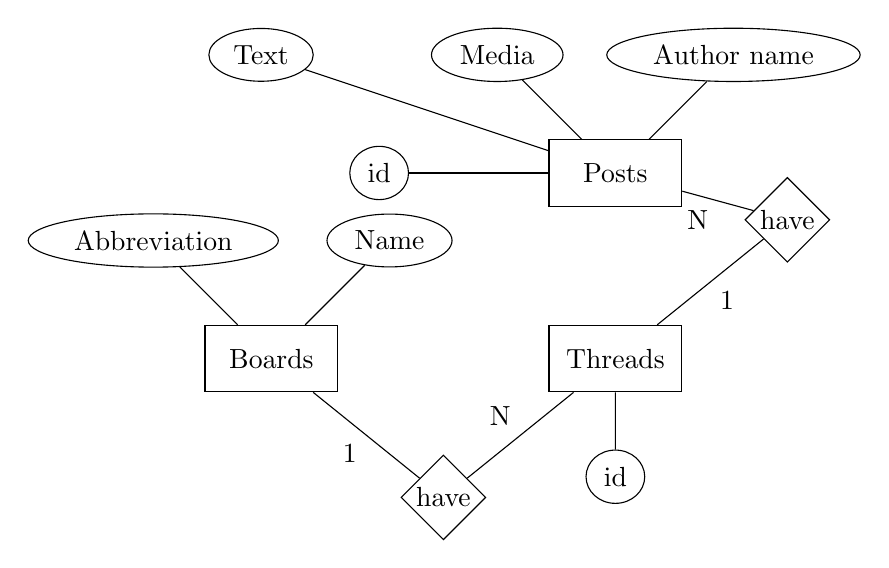
\begin{tikzpicture}[auto,node distance=1.5cm]
        \node[entity] (board_node) {Boards}
            [grow=up,sibling distance=3cm]
            child {node[attribute] {Name}}
            child {node[attribute] {Abbreviation}};
        \node[relationship] (board_thread) [below right = of board_node] {have};
        \node[entity] (thread_node) [above right = of board_thread]	{Threads}
            child {node[attribute] {id}};
        \path (board_thread) edge node {1} (board_node) edge node {N} (thread_node);
        \node[entity] (post_node) [above = of thread_node] {Posts}
            [grow=up,sibling distance=3cm]
            child[grow=left,level distance=3cm] {node[attribute] {id}}
            child {node[attribute] {Author name}}
            child {node[attribute] {Media}}
            child {node[attribute] {Text}};
        \node[relationship] (thread_post) [above right = of thread_node] {have};
        \path (thread_post) edge node {1} (thread_node) edge node {N} (post_node);
    \end{tikzpicture}
    \caption{
        Diagrama entidade-relacional demonstrando um modelo de dados de alto nível do 4chan.\\
        Fonte: os autores.
    }
    \label{fig:er-4chan}
\end{figure}

\subsection{Banco de dados}

Para o nosso banco de dados, escolhemos o que há de mais portátil e acessível: o sistema de arquivos.
Os dados colaboram para isso, pois não têm nenhuma relação com cardinalidade que nos impeça de modelá-los denormalizados, então assim o fizemos. Como pode ser visto na árvore de diretórios na \textbf{figura X}, temos:

\begin{itemize}
    \item Uma pasta raíz com N subpastas, cada um correspondendo a um board.
    \item Cada pasta de board, identificada pela abreviação única do board, possui N subpastas e cada uma dessas corresponde a uma thread.
    \item Cada pasta de thread possui 
        \subitem uma subpasta \code{media} onde todas imagens e vídeos da thread são armazenados;
        \subitem um arquivo \code{thread.json} onde todos dados pertinentes àquela thread são armazenados.
\end{itemize}

% \begin{verbatim}
% $ tree 4chan-archive/
% └── w/
%     ├── 2131136/
%     │   ├── media/
%     │   │   ├── 1600798279711.png
%     │   │   ├── 1600814639570.jpg
%     │   │   └── ...
%     │   └── thread.json
%     ├── 2180136/
%     │   ├── media/
%     │   └── thread.json
%     └── 2180395/
%         ├── media/
%         └── thread.json
% \end{verbatim}


\chapter{Modelagem do Sistema}

Este capítulo apresenta a modelagem completa das ferramentas
propostas, buscando o esclarecimento de suas funcionalidades e características
através de sua abstração.

\section{Diagramas de Atividades}

Nesta seção serão apresentados os diagramas de atividade das ferramentas quem tem contato direto com o usuário(\textit{Scraper} e Rede \textit{Peer-to-Peer}), com foco nas atividades que serão executadas no funcionamento destas ferramentas.
\subsection{Extração de Dados\label{subsec:extracao_de_dados}}
Esse processo realiza a extração de dados da web 2.0, esse é o método principal para a migração de dados da web 2.0 para a web 3.0, as principais atividade do processo podem ser vistas no diagrama de atividades representado na figura ~\ref{fig:extracao_de_dados}.
\begin{figure}[H]
    \centering
    \includesvg[width=\textwidth]{fig/Extracao_de_dados.svg}
    \caption[Diagrama de Atividades : Extração de Dados]{\label{fig:extracao_de_dados}
        Diagrama de Atividades : Extração de Dados\\
        Fonte: os autores.
    }
\end{figure}
Esse processo já está descrito a partir da rede social da web 2.0 que será utilizada para a aplicação das ferramentas deste trabalho, assim além
do usuário e da ferramenta \textit{scraper} temos a API do \textit{4chan}. Por estarmos utilizando o \textit{4chan} que é uma plataforma que não necessita o cadastro de um usuário não existe o passo para a autenticação junto a API, para outras plataformas como \textit{Facebook} e \textit{Twitter} necessitaríamos um passo a mais e a utilização  de um \textit{token} nas chamadas a API.

O processo começa com a etapa onde o usuário indica qual o dado deseja salvar em seu computador; Exemplo: \textit{board}, \textit{thread}, comentário (Todos exemplos de postagens do \textit{4chan}). E depois o
formato que deseja que eles sejam salvos; Exemplo: XML, JSON, TXT. Após essa primeira etapa o \textit{scraper} recebe esses dados e cria uma requisição para a API do \textit{4chan} e fica no aguardo da
reposta, recebido a resposta o \textit{scraper} formata os dados conforme os parametros que o usuário especificou e salva os dados no local indicado pelo usuário.

\subsection{Solicitação de Dados pela Rede P2P\label{subsec:Solicitacao_Dados}}
Este processo realiza a comunicação e a troca de dados dentro da rede P2P, uma fez extraído os dados da web 2.0 esse vai ser o novo formato de obtenção e troca de dados sem a necessidade do 
do \textit{4chan}. A partir deste processo o usuário fica independente das plataformas da web 2.0. as principais atividade do processo podem ser vistas no diagrama de atividades 
representado na figura ~\ref{fig:Solicitacao_Dados}. 
\begin{figure}[H]
    \includesvg[width= 1.11\textwidth]{fig/Solicitacao_Dados.svg}
    \caption[Diagrama de Atividades : Solicitação de Dados pela Rede P2P]{\label{fig:Solicitacao_Dados}
        Diagrama de Atividades : Solicitação de Dados pela Rede P2P\\
        Fonte: os autores.
    }
\end{figure}
O processo começa com a etapa onde o usuário indica qual o dado deseja acessar; Exemplo:\textit{board}, \textit{thread}, comentário (Todos exemplos de postagens do \textit{4chan}). Depois a rede procura pela \textit{hash} desse \textit{post} na rede para descobrir qual nodo tem esse dado, verificando-se existem nodos da lista de nodos confiáveis do usuário, não tendo nodos da lista confiáveis oferece a opção de baixar
de um nodo não confiável. Após essa primeira etapa é realizado a comunicação entre os nodos e transferido os arquivos, por fim o usuário escolhe se deseja manter salvo os arquivos 
em usa máquina. 
\section{Diagramas de Sequência}
Nesta seção serão apresentados os diagramas de sequencia das ferramentas quem tem contato direto com o usuário(\textit{Scraper} e Rede \textit{Peer-to-Peer}), com foco na comunicação entre os objetos e nos tempos de execução e reposta das funcionalidade destas ferramentas.
\subsection{Extração de Dados}
Esta seção faz a analise dos tempos de execução e resposta do processo de extração de dados descrito na seção~\ref{subsec:extracao_de_dados}. A representação dos tempos de execução podem ser vistas através do diagrama de sequencia representado na figura~\ref{fig:seq_extracao_dados}. 
\begin{figure}[H]
    \includesvg[width= 1.10\textwidth]{fig/DiagramadeSequenciaScraper.svg}
    \caption[Diagrama de Sequência : Extração de Dados]{\label{fig:seq_extracao_dados}
        Diagrama de Sequência : Extração de Dados\\
        Fonte: os autores.
    }
\end{figure}

O processo inicia com a solicitação síncrona do usuário ao \textit{Scraper}, que envia uma requisição síncrona para a API do \textit{4chan}, o \textit{Scraper} fica a espera de uma resposta assíncrona do \textit{4chan} e envia uma resposta assíncrona para o usuário. 
O tempo de espera do usuário deve ser perto do tempo de espera de uma aplicação da web 2.0, visto que o processo é o mesmo. A única diferença de tempo que pode ser esperada depende do formato do dado que o usuário escolheu
se o formato for diferente da resposta da API um tempo de formatação do \textit{Scraper} deverá ser adicionado ao tempo de espera esperado.

\subsection{Solicitação de Dados pela Rede P2P}
Esta seção faz a analise dos tempos de execução e resposta do processo de solicitação de dados pela \textit{rede peer-to-peer} descrito na seção~\ref{subsec:Solicitacao_Dados}. A representação dos tempos de execução podem ser vistas através do diagrama de sequencia representado na figura~\ref{fig:seq_Solicitacao_dados}. 
\begin{figure}[H]
    \includesvg[width= 1.11\textwidth]{fig/DiagramaSequenciaRedeP2P.svg}
    \caption[Diagrama de Sequência :Solicitação de Dados pela Rede P2P]{\label{fig:seq_Solicitacao_dados}
        Diagrama de Sequência : Solicitação de Dados pela Rede P2P\\
        Fonte: os autores.
    }
\end{figure}
O processo inicia com solicitação síncrona do usuário a rede \textit{peer-to-peer}, indicando os dados
requisitados, a rede \textit{peer-to-peer} envia uma resposta assíncrona que pode ser dado encontrado ou dado não encontrado,
a partir desse dado o usuário envia uma solicitação ao \textit{peer} que contém o conteúdo desejado
e começa o download do conteúdo. Este processo contém algumas variáveis, como a conexão entre os dois \textit{peers}
e quantos \textit{peers} na rede contém aquele dado, pois na rede \textit{peer-to-peer} é possível baixar partes de um dado de fontes diferentes. Assim o tempo de execução pode ser menor ou maior que o da plataforma da web 2.0.
\section{Diagramas de Casos de Uso}
Nesta seção serão apresentados os diagramas de caso de uso e os atores
modelados por ferramenta. O objetivo do uso desta modelagem é abordar mais profundamente as funcionalidades das ferramentas atráves da modelagem de casos de uso. 
\subsection{Atores}
Por o projeto ser um conjunto de ferramentas, elas serão utilizadas apenas por um tipo de Ator, o usuário. Ele será responsável por fornecer os dados de entrada para as ferramentas, e as configurações que melhor desejar e que possam ser fornecidas as ferramentas.
\begin{figure}[H]
    \centering
    \includesvg[width=0.09\textwidth]{fig/Ator.svg}
    \caption[Diagrama do Ator]{\label{fig:diagrama_do_ator}
        Diagrama do Ator\\
        Fonte: os autores.
    }
\end{figure}
\subsection{Casos de Uso Scraper}
Nesta seção será apresentado os casos de uso para o ator usuário na ferramenta \textit{Scraper}.
\subsubsection{UC01 - Especificar o Formato dos Dados}
Permite ao usuário especificar ao \textit{Scraper} qual o formato dos dados que ele espera receber. Para isso o usuário deve passar como parâmetro para o \textit{Scraper} essa informação, ou configurá-lo previamente com o formato favorito.
\subsubsection{UC02 - Baixar conteúdo de Texto de uma Thread do 4chan}
Permite ao usuário baixar todo o texto de uma thread do 4chan. Para isso o usuário deve passar como parâmetro para o \textit{Scraper} a id da thread que deseja baixar o texto.
\subsubsection{UC03 - Baixar conteúdo de mídia(fotos, vídeos)  de uma Thread do 4chan}
Permite ao usuário baixar todo a mídia de uma thread do 4chan. Para isso o usuário deve passar como parâmetro para o \textit{Scraper} a id da thread que deseja baixar a mídia.
\subsubsection{UC04 - Baixar todo o conteúdo de uma Thread do 4chan}
Permite ao usuário baixar todo a conteúdo de uma thread do 4chan (mídia e texto). Para isso o usuário deve passar como parâmetro para o \textit{Scraper} a id da thread que deseja baixar todo o conteúdo.
\begin{figure}[ht]
    \centering
    \includesvg[width=\textwidth]{fig/Ator_Scraper1.svg}
    \caption[Casos de uso Scraper UC01, UC02, UC03, e UC04]{\label{fig:Ator_Scraper1}
        Casos de uso Scraper UC01,UC02,UC03,UC04\\
        Fonte: os autores.
    }
\end{figure}
\subsubsection{UC05 - Especificar Threads para monitoramento}
Permite ao usuário informar uma thread para monitoramento no 4chan, assim o scraper fará consultas constantemente, buscando e baixando alterações na thread. Para isso o usuário deve passar como parâmetro para o \textit{Scraper} a id da thread que deseja monitorar.  
\subsubsection{UC06 - Especificar Boards para monitoramento}
Permite ao usuário informar um board para monitoramento no 4chan, assim o scraper fará consultas constantemente, buscando e baixando alterações no board. Para isso o usuário deve passar como parâmetro para o \textit{Scraper} a id do board que deseja monitorar.  
\subsubsection{UC07 - Interromper o monitoramento de uma Thread que estiver fechada}
Permite ao usuário configurar o \textit{Scraper} para parar de monitorar threads que estiverem fechadas.
\begin{figure}[H]
    \centering
    \includesvg[width=0.65\textwidth]{fig/Ator_Scraper2.svg}
    \caption[Casos de uso Scraper UC05,UC06,UC07]{\label{fig:Ator_Scraper2}
        Casos de uso Scraper UC05,UC06,UC07\\
        Fonte: os autores.
    }
\end{figure}
\subsection{Casos de Uso Networking}
Nesta seção será apresentado os casos de uso para o ator usuário com ferramenta \textit{Networking}.
\subsubsection{UC01 - Procurar Conteúdo pela Rede}
Permite ao usuário procurar conteúdo pela rede peer-to-peer, para isso ele deve passar o nome ou hash do arquivo que deseja.
\subsubsection{UC02 - Requisitar Conteúdo pela Rede}
Permite ao usuário requisitar conteúdo pela rede peer-to-peer, para isso ele deve passar o nome ou hash do arquivo que deseja.
\subsubsection{UC03 - Fornecer Conteúdo pela Rede}
Permite ao usuário fornecer conteúdo pela rede peer-to-peer, para isso ele deve ter o arquivo e configurar a rede para fornecer o conteúdo.
\begin{figure}[H]
    \centering
    \includesvg[width=0.5\textwidth]{fig/Ator_Networking1.svg}
    \caption[Casos de uso Networking UC01,UC02,UC03]{\label{fig:Ator_Networking2}
        Casos de uso Networking UC01,UC02,UC03\\
        Fonte: os autores.
    }
\end{figure}
\subsection{Casos de Uso Criptografia}
Nesta seção será apresentado os casos de uso para o ator usuário com ferramenta \textit{Criptografia}.
\subsubsection{UC01 - Criar um par de chaves criptográficas}
Permite ao usuário criar um par de chaves criptográficas para garantir a autenticidade e integridade no compartilhamento de arquivos na rede.
\subsubsection{UC02 - Criar lista de nodos confiáveis}
Permite ao usuário criar uma lista de nodos confiáveis, para isso o usuário deve armazenar uma lista com a chave pública dos nodos que julgar confiáveis.
\subsubsection{UC03 - Exportar minha chave pública para Compartilhamento}
Permite ao usuário exportar a chave pública no formato cleartext para compartilhamento. Para isso o usuário necessita ter um par de chaves criptográficas. 
\begin{figure}[H]
    \centering
    \includesvg[width=0.7\textwidth]{fig/Ator_Crypto1.svg}
    \caption[Casos de uso Criptografia UC01,UC02,UC03]{\label{fig:Ator_Crypto1}
        Casos de uso Criptografia UC01,UC02,UC03\\
        Fonte: os autores.
    }
\end{figure}
\subsubsection{UC04 - Assinar arquivos com a minha chave privada}
Permite ao usuário assinar arquivos com sua chave privada para que os outros peers da rede que o mantém como nodo confiável e tem sua chave publica possam reconhecer a assinatura e identificar que ele é um peer confiável. Para isso o usuário deve ter um par de chaves criptográficas.
\subsubsection{UC05 - Verificar se a assinatura de um arquivo pertence a minha lista de nodos confiáveis}
Permite ao usuário identificar a assinatura de um nodo confiável a partir da chave publica na lista de nodos confiáveis. Para isso o usuário necessita ter armazenado na sua lista de nodos confiáveis a chave publica do nodo.
\begin{figure}[H]
    \centering
    \includesvg[width=0.7\textwidth]{fig/Ator_Crypto2.svg}
    \caption[Casos de uso Criptografia UC04,UC05]{\label{fig:Ator_Crypto2}
        Casos de uso Criptografia UC04,UC05\\
        Fonte: os autores.
    }
\end{figure}
\section{Detalhamento dos Casos de Uso}

\subsection{Especificar o Formato dos Dados}
\subsubsection{Descrição}
Permite ao usuário especificar ao \textit{Scraper} qual o formato dos dados que ele espera receber. Para isso o usuário deve passar como parâmetro para o \textit{Scraper} essa informação, ou configurá-lo previamente com o formato favorito.
\subsubsection{Atores : Usuário}
\subsubsection{Pré-Condição}
O usuário deve informar o formato dos dados.
\subsubsection{Pós-Condição}
O usuário tem o dados no formato desejado.
\subsubsection{Fluxo Principal}
\begin{enumerate}
    \item Abre o Scraper pela linha de comando;
    \item Passa como parâmetro o id do dado que deseja e o formato dos dados;
    \item Scraper realiza a busca do dado;
    \item Scraper realiza a formatação do dado;
    \item O usuário abre o dado;
\end{enumerate}
\subsubsection{Fluxo Alternativo}
\begin{itemize}
    \item Dado não existe no 4chan: ocorre quando no passo 3 scraper não acha o dado indicado pelo usuário no 4chan.
    \begin{enumerate}
        \item Mostra mensagem de erro;
        \item Retorna ao passo 2.
    \end{enumerate}
    \item Scraper não reconhece o formato especificado: ocorre quando no passo 4 o scraper vai formatar o dado indicado pelo usuário e não consegue identificar o formato desejado.
    \begin{enumerate}
        \item Mostra mensagem de erro;
        \item Retorna ao passo 2.
    \end{enumerate}
\end{itemize}


\subsection{Baixar conteúdo de Texto de uma Thread do 4chan}
\subsubsection{Descrição}
Permite ao usuário baixar todo o texto de uma thread do 4chan. Para isso o usuário deve passar como parâmetro para o \textit{Scraper} a id da thread que deseja baixar o texto.
\subsubsection{Atores : Usuário}
\subsubsection{Pré-Condição}
O usuário deve informar o id das threads que deseja salvar.
\subsubsection{Pós-Condição}
O usuário terá o todo conteúdo de texto da thread indicada.
\subsubsection{Fluxo Principal}
\begin{enumerate}
    \item Abre o Scraper pela linha de comando;
    \item Passa como parâmetro o id do dado que deseja e o formato dos dados;
    \item Scraper realiza a busca do dado;
    \item Scraper realiza a formatação do dado;
    \item O usuário abre o dado;
\end{enumerate}
\subsubsection{Fluxo Alternativo}
\begin{itemize}
    \item Dado não existe no 4chan: ocorre quando no passo 3 scraper não acha o dado indicado pelo usuário no 4chan.
    \begin{enumerate}
        \item Mostra mensagem de erro;
        \item Retorna ao passo 2.
    \end{enumerate}
    \item Scraper não reconhece o formato especificado: ocorre quando no passo 4 o scraper vai formatar o dado indicado pelo usuário e não consegue identificar o formato desejado.
    \begin{enumerate}
        \item Mostra mensagem de erro;
        \item Retorna ao passo 2.
    \end{enumerate}
\end{itemize}

\subsection{Baixar conteúdo de mídia de uma Thread do 4chan}
\subsubsection{Descrição}
Permite ao usuário baixar todo a mídia de uma thread do 4chan. Para isso o usuário deve passar como parâmetro para o \textit{Scraper} a id da thread que deseja baixar a mídia.
\subsubsection{Atores : Usuário}
\subsubsection{Pré-Condição}
O usuário deve informar o id das threads que deseja salvar.
\subsubsection{Pós-Condição}
O usuário terá o todo conteúdo de mídia(fotos,vídeos) da thread indicada.
\subsubsection{Fluxo Principal}
\begin{enumerate}
    \item Abre o Scraper pela linha de comando;
    \item Passa como parâmetro o id do dado que deseja e o formato dos dados;
    \item Scraper realiza a busca do dado;
    \item Scraper realiza a formatação do dado;
    \item O usuário abre o dado;
\end{enumerate}
\subsubsection{Fluxo Alternativo}
\begin{itemize}
    \item Dado não existe no 4chan: ocorre quando no passo 3 scraper não acha o dado indicado pelo usuário no 4chan.
    \begin{enumerate}
        \item Mostra mensagem de erro;
        \item Retorna ao passo 2.
    \end{enumerate}
    \item Scraper não reconhece o formato especificado: ocorre quando no passo 4 o scraper vai formatar o dado indicado pelo usuário e não consegue identificar o formato desejado.
    \begin{enumerate}
        \item Mostra mensagem de erro;
        \item Retorna ao passo 2.
    \end{enumerate}
\end{itemize}

\subsection{Baixar todo o conteúdo de uma Thread do 4chan}
\subsubsection{Descrição}
Permite ao usuário baixar todo a conteúdo de uma thread do 4chan (mídia e texto). Para isso o usuário deve passar como parâmetro para o \textit{Scraper} a id da thread que deseja baixar todo o conteúdo.
\subsubsection{Atores : Usuário}
\subsubsection{Pré-Condição}
O usuário deve informar o id das threads que deseja salvar.
\subsubsection{Pós-Condição}
O usuário terá o todo conteúdo da thread indicada.
\subsubsection{Fluxo Principal}
\begin{enumerate}
    \item Abre o Scraper pela linha de comando;
    \item Passa como parâmetro o id do dado que deseja e o formato dos dados;
    \item Scraper realiza a busca do dado;
    \item Scraper realiza a formatação do dado;
    \item O usuário abre o dado;
\end{enumerate}
\subsubsection{Fluxo Alternativo}
\begin{itemize}
    \item Dado não existe no 4chan: ocorre quando no passo 3 scraper não acha o dado indicado pelo usuário no 4chan.
    \begin{enumerate}
        \item Mostra mensagem de erro;
        \item Retorna ao passo 2.
    \end{enumerate}
    \item Scraper não reconhece o formato especificado: ocorre quando no passo 4 o scraper vai formatar o dado indicado pelo usuário e não consegue identificar o formato desejado.
    \begin{enumerate}
        \item Mostra mensagem de erro;
        \item Retorna ao passo 2.
    \end{enumerate}
\end{itemize}


\subsection{Especificar Threads para monitoramento}
\subsubsection{Descrição}
Permite ao usuário informar uma thread para monitoramento no 4chan, assim o scraper fará consultas constantemente, buscando e baixando alterações na thread. Para isso o usuário deve passar como parâmetro para o \textit{Scraper} a id da thread que deseja monitorar. 
\subsubsection{Atores : Usuário}
\subsubsection{Pré-Condição}
O usuário deve informar o id das threads que deseja monitorar.
\subsubsection{Pós-Condição}
O usuário terá o conteúdo da thread constantemente atualizado.
\subsubsection{Fluxo Principal}
\begin{enumerate}
    \item Abre o Scraper pela linha de comando;
    \item Passa como parâmetro o id da thread que deseja monitorar;
    \item Scraper realiza a busca da thread;
    \item Scraper começa o monitoramento da thread;
\end{enumerate}
\subsubsection{Fluxo Alternativo}
\begin{itemize}
    \item Thread não existe no 4chan: ocorre quando no passo 3 scraper não acha a thread indicado pelo usuário no 4chan.
    \begin{enumerate}
        \item Mostra mensagem de erro;
        \item Retorna ao passo 2.
    \end{enumerate}
\end{itemize}


\subsection{Especificar Boards para monitoramento}
\subsubsection{Descrição}
Permite ao usuário informar um board para monitoramento no 4chan, assim o scraper fará consultas constantemente, buscando e baixando alterações no board. Para isso o usuário deve passar como parâmetro para o \textit{Scraper} a id do board que deseja monitorar.  
\subsubsection{Atores : Usuário}
\subsubsection{Pré-Condição}
O usuário deve informar o id das boards que deseja monitorar.
\subsubsection{Pós-Condição}
O usuário terá o conteúdo do board constantemente atualizado.
\subsubsection{Fluxo Principal}
\begin{enumerate}
    \item Abre o Scraper pela linha de comando;
    \item Passa como parâmetro o id do board que deseja monitorar;
    \item Scraper realiza a busca do board;
    \item Scraper começa o monitoramento do board;
\end{enumerate}
\subsubsection{Fluxo Alternativo}
\begin{itemize}
    \item Board não existe no 4chan: ocorre quando no passo 3 scraper não acha o board indicado pelo usuário no 4chan.
    \begin{enumerate}
        \item Mostra mensagem de erro;
        \item Retorna ao passo 2.
    \end{enumerate}
\end{itemize}


\subsection{Interromper o monitoramento de uma Thread que estiver fechada}
\subsubsection{Descrição}
Permite ao usuário configurar o \textit{Scraper} para parar de monitorar threads que estiverem fechadas.
\subsubsection{Atores : Usuário}
\subsubsection{Pré-Condição}
Nenhuma pré-condição é necessária.
\subsubsection{Pós-Condição}
O scraper deixará de buscar atualizações na thread.
\subsubsection{Fluxo Principal}
\begin{enumerate}
    \item Abre o Scraper pela linha de comando;
    \item Passa como parâmetro o id da thread;
    \item Scraper adiciona ao monitoramento da thread a flag de fechada ou aberto;
\end{enumerate}
\subsubsection{Fluxo Alternativo}
\begin{itemize}
    \item Thread não existe no 4chan: ocorre quando no passo 3 scraper não acha a Thread indicado pelo usuário no 4chan.
    \begin{enumerate}
        \item Mostra mensagem de erro;
        \item Retorna ao passo 2.
    \end{enumerate}
    \item Scraper não monitora essa thread: ocorre quando no passo 3 scraper não tem essa Thread na sua lista de monitoração.
    \begin{enumerate}
        \item Mostra mensagem de erro;
        \item Retorna ao passo 2.
    \end{enumerate}
\end{itemize}


\subsection{Procurar Conteúdo pela Rede}
\subsubsection{Descrição}
Permite ao usuário procurar conteúdo pela rede peer-to-peer, para isso ele deve passar o nome ou hash do arquivo que deseja.
\subsubsection{Atores : Usuário}
\subsubsection{Pré-Condição}
O usuário deve informar o nome ou a hash do arquivo que deseja buscar.
\subsubsection{Pós-Condição}
O usuário saberá se um dado existe na rede, e os nodos que contem aquele dado.
\subsubsection{Fluxo Principal}
\begin{enumerate}
    \item Se conecta a rede pela linha de comando;
    \item Passa como parâmetro o nome ou hash do arquivo desejado;
    \item A rede pesquisa o arquivo pela rede;
    \item A rede informa uma lista de usuário que contém o arquivo;
\end{enumerate}
\subsubsection{Fluxo Alternativo}
\begin{itemize}
    \item O arquivo não existe na rede: ocorre quando no passo 3 a rede não acha o arquivo indicado pelo usuário.
    \begin{enumerate}
        \item Mostra mensagem de erro;
        \item Retorna ao passo 2.
    \end{enumerate}
\end{itemize}


\subsection{Requisitar Conteúdo pela Rede}
\subsubsection{Descrição}
Permite ao usuário requisitar conteúdo pela rede peer-to-peer, para isso ele deve passar o nome ou hash do arquivo que deseja.
\subsubsection{Atores : Usuário}
\subsubsection{Pré-Condição}
O usuário deve informar o nome ou a hash do arquivo que deseja requisitar.
\subsubsection{Pós-Condição}
O usuário terá o arquivo requisitado.
\subsubsection{Fluxo Principal}
\begin{enumerate}
    \item Se conecta a rede pela linha de comando;
    \item Passa como parâmetro o nome ou hash do arquivo desejado;
    \item A rede pesquisa o arquivo pela rede;
    \item A rede informa uma lista de usuário que contém o arquivo;
    \item O usuário informa se conecta a um dos usuários da lista;
    \item O usuário baixa o arquivo desejado;
\end{enumerate}
\subsubsection{Fluxo Alternativo}
\begin{itemize}
    \item O arquivo não existe na rede: ocorre quando no passo 3 a rede não acha o arquivo indicado pelo usuário.
    \begin{enumerate}
        \item Mostra mensagem de erro;
        \item Retorna ao passo 2.
    \end{enumerate}
    \item Não existe peers Confiáveis: ocorre quando no passo 4 nenhum dos peers está na lista de confiáveis do usuário.
    \begin{enumerate}
        \item Mostra mensagem se o usuário deseja prosseguir com um peer não confiável;
        \item Segue ao passo 5 ou encerra a execução.
    \end{enumerate}
\end{itemize}


\subsection{Fornecer Conteúdo pela Rede}

\subsubsection{Descrição}

Permite ao usuário fornecer conteúdo pela rede peer-to-peer, para isso ele deve ter o arquivo e configurar a rede para fornecer o conteúdo.

\subsubsection{Atores : Usuário}

\subsubsection{Pré-Condição}

O usuário deve ter armazenado os arquivos que deseja fornecer.

\subsubsection{Pós-Condição}

O usuário estará disponível na para outros usuários quando pesquisarem pelo arquivo servido. 

\subsubsection{Fluxo Principal}

\begin{enumerate}
    \item Se conecta a rede pela linha de comando;
    \item Passa como parâmetro o local do arquivo em sua maquina;
    \item A rede lê o arquivo;
    \item A rede gera uma hash e espoem o arquivo para a rede;
\end{enumerate}

\subsubsection{Fluxo Alternativo}

\begin{itemize}
    \item O arquivo não existe no caminho informado: ocorre quando no passo 3 a rede não acha o arquivo indicado pelo usuário.
    \begin{enumerate}
        \item Mostra mensagem de erro;
        \item Retorna ao passo 2.
    \end{enumerate}
\end{itemize}


\subsection{Criar um par de chaves criptográficas}
\subsubsection{Descrição}
Permite ao usuário criar um par de chaves criptográficas para garantir a autenticidade e integridade no compartilhamento de arquivos na rede.
\subsubsection{Atores : Usuário}
\subsubsection{Pré-Condição}
Nenhuma pré-condição é necessária.
\subsubsection{Pós-Condição}
O usuário terá um chave pública e uma chave criptográfica.
\subsubsection{Fluxo Principal}
\begin{enumerate}
    \item Se conecta ao modulo de criptografia pela linha de comando;
    \item Executa o método para criação de chaves criptográficas;
    \item O modulo de criptografia gera um par de chaves criptográficas para o usuário;
\end{enumerate}


\subsection{Criar lista de nodos confiáveis}
\subsubsection{Descrição}
Permite ao usuário criar uma lista de nodos confiáveis, para isso o usuário deve armazenar uma lista com a chave pública dos nodos que julgar confiáveis.
\subsubsection{Atores : Usuário}
\subsubsection{Pré-Condição}
O usuário deve ter no mínimo uma chave publica de um nodo para criar a lista.
\subsubsection{Pós-Condição}
O usuário terá uma lista de nodos confiáveis que poderá ser usado para verificar a identidade de um usuário e auxiliar no download de dados pela rede.
\subsubsection{Fluxo Principal}
\begin{enumerate}
    \item Se conecta a rede pela linha de comando;
    \item Executa o método para criação de lista de nodos confiáveis passando como parâmetro a chave publica de um nodo confiável;
    \item A rede gera a lista de nodos confiáveis;
\end{enumerate}
\subsubsection{Fluxo Alternativo}
\begin{itemize}
    \item A lista já foi criada: ocorre quando no item 3 já ter uma lista criada.
    \begin{enumerate}
        \item Mostra mensagem de erro, perguntado se deseja substituir a lista;
        \item Substitui a lista ou encerra o programa.
    \end{enumerate}
\end{itemize}


\subsection{Exportar minha chave pública para Compartilhamento}
\subsubsection{Descrição}
Permite ao usuário exportar a chave pública no formato cleartext para compartilhamento. Para isso o usuário necessita ter um par de chaves criptográficas. 
\subsubsection{Atores : Usuário}
\subsubsection{Pré-Condição}
O usuário precisa ter chaves criptográficas.
\subsubsection{Pós-Condição}
O usuário terá sua chave publica num formato de fácil compartilhamento.
\subsubsection{Fluxo Principal}
\begin{enumerate}
    \item Se conecta a rede pela linha de comando;
    \item Executa o método para exportar a chave publica no formato cleartext;
    \item A rede gera a converte a chave publica para cleartext e informa ao usuário;
\end{enumerate}
\subsubsection{Fluxo Alternativo}
\begin{itemize}
    \item O usuário não tem chave publica cadastrada: ocorre quando no item 3 o usuário não tem um par de chaves criptográficas criadas.
    \begin{enumerate}
        \item Mostra mensagem de erro;
        \item Encerra o programa.
    \end{enumerate}
\end{itemize}


\subsection{Assinar arquivos com a minha chave privada}
\subsubsection{Descrição}
Permite ao usuário assinar arquivos com sua chave privada para que os outros peers da rede que o mantém como nodo confiável e tem sua chave publica possam reconhecer a assinatura e identificar que ele é um peer confiável. Para isso o usuário deve ter um par de chaves criptográficas.
\subsubsection{Atores : Usuário}
\subsubsection{Pré-Condição}
O usuário precisa ter chaves criptográficas.
\subsubsection{Pós-Condição}
O arquivo poderá ser verificado por usuários que tenham a chave pública correspondente.
\subsubsection{Fluxo Principal}
\begin{enumerate}
    \item Se conecta a rede pela linha de comando;
    \item Executa o método para assinar um arquivo passando como parâmetro o caminho do arquivo na maquina do usuário;
    \item A rede gera uma assinatura no arquivo;
\end{enumerate}
\subsubsection{Fluxo Alternativo}
\begin{itemize}
    \item O usuário não tem chave publica cadastrada: ocorre quando no item 3 o usuário não tem um par de chaves criptográficas criadas.
    \begin{enumerate}
        \item Mostra mensagem de erro;
        \item Encerra o programa.
    \end{enumerate}
     \item O arquivo não existe: ocorre quando no item 3 o programa não acha o arquivo no caminho especificado pelo usuário.
    \begin{enumerate}
        \item Mostra mensagem de erro;
        \item Retorna ao passo 2.
    \end{enumerate}
\end{itemize}

\subsection{Verificar se a assinatura de um arquivo pertence a minha lista de nodos confiáveis}
\subsubsection{Descrição}
Permite ao usuário identificar a assinatura de um nodo confiável a partir da chave publica na lista de nodos confiáveis. Para isso o usuário necessita ter armazenado na sua lista de nodos confiáveis a chave publica do nodo.
\subsubsection{Atores : Usuário}
\subsubsection{Pré-Condição}
O usuário precisa ter uma lista de nodos confiáveis.
\subsubsection{Pós-Condição}
O usuário terá verificado a identidade de quem assinou aquele arquivo.
\subsubsection{Fluxo Principal}
\begin{enumerate}
    \item Se conecta a rede pela linha de comando;
    \item Executa o método para buscar um arquivo na passando como parâmetro o nome ou a hash do arquivo;
    \item A rede pesquisa o arquivo pela rede;
    \item A rede informa uma lista de usuário que contém o arquivo;
    \item O usuário seleciona o arquivo e usuário e pede para rede verificar a assinatura;
    \item A rede verifica a assinatura.
\end{enumerate}
\subsubsection{Fluxo Alternativo}
\begin{itemize}
    \item O arquivo não existe na rede: ocorre quando no passo 3 a rede não acha o arquivo indicado pelo usuário.
    \begin{enumerate}
        \item Mostra mensagem de erro;
        \item Retorna ao passo 2.
    \end{enumerate}
\end{itemize}


\chapter{Metodologia}

A metodologia empregada para o planejamento e desenvolvimento do sistema deste trabalho de conclusão é o tradicional modelo cascata.
Esse modelo funciona como um exemplo de um processo dirigido a planos, onde, em princípio deve-se planejar e programar todas as atividades do processo até a implementação e a manutenção do dele~\cite{SOMMERVILLE1}.

Consiste numa sequência de fases em que cada fase dá suporte para a próxima, assim o produto de cada fase torna-se a entrada para a seguinte~\cite{BALTZAN1}, a fase inicial é definição de requisitos que busca estabelecer os serviços, restrições e metas do sistema, normalmente por meio de consultas com o usuário~\cite{SOMMERVILLE1}; a próxima fase projeto de sistema e software é a fase em que a identificação e descrição das abstrações fundamentais do sistema é realizada, alocando os requisitos do sistema por meio de uma arquitetura geral do sistema~\cite{SOMMERVILLE1}; a terceira fase implementação e teste unitário é a fase de desenvolvimento do projeto como um conjunto de programas ou unidades de programa, utilizando o teste unitário para verificar de cada unidade, tendo certeza de que a mesma cumpra sua especificação~\cite{SOMMERVILLE1}; a quarta fase integração e teste de sistema é quando as unidades criadas na fase anterior de maneira independente são integradas e testadas como um sistema único e completo, verificando se todos os requisitos estão sendo atendidos~\cite{SOMMERVILLE1}.
Na fase final, Operação e manutenção, é o momento em que o sistema é de fato instalado e colocado em uso, é onde os eventuais erros que não apareceram anteriormente são resolvidos e, também, onde novos requisitos podem ser descobertos~\cite{SOMMERVILLE1}. 
\begin{figure}[H]
    \centering
    \includesvg[width=\textwidth]{fig/Modelo_Cascata.svg}
    \caption[Diagrama do Modelo Cascata]{\label{fig:Modelo_Cascata}
        Diagrama do Modelo Cascata\\
        Fonte: os autores.
    }
\end{figure}
Por mais que essa seja uma metodologia não mais tão utilizada pelas empresas devido à sua característica de precisão extrema que não leva em consideração mudanças durante o desenvolvimento do projeto~\cite{BALTZAN1}, para este trabalho ela se torna uma boa escolha, pois se trata de um Trabalho de Conclusão de Curso, com um único desenvolvedor e prazos muito bem definidos.
Devido à inexistência de um cliente e visando um público alvo, reuniões com o cliente são impossíveis e testes durante o desenvolvimento do trabalho com alguém que faça parte do público alvo não acontecerão facilmente, o modelo cascata se torna a melhor opção como metodologia de desenvolvimento do projeto. A partir de agora as fases alvo são: a codificação, os testes e a implementação/manutenção do sistema, concluindo assim o ciclo completo do modelo tradicional em cascata.
\chapter{Cronograma}

Apresentamos a seguir um cronograma relatando nossas atividades desenvolvidas e nosso planejamento, relatando as atividades que já foram e que serão desenvolvidas.

\begin{enumerate}
    \item \label{cron:search} Seleção e análise das redes sociais atuais.
        \subitem Mapear vantagens e desvantagens delas.
    \item \label{cron:background} Consolidação da fundamentação teórica.
    \item \label{cron:architecture} Elaboração da proposta de Arquitetura.
    \item \label{cron:proposal} Entrega da proposta de TC.
    \item \label{cron:requirements} Identificação dos requisitos do sistema.
    \item \label{cron:diagrams} Elaboração da modelagem do sistema.
    \item \label{cron:methodology} Definição da metodologia de desenvolvimento.
    \item \label{cron:esc-tcI} Entrega do volume final de TC1.
    \item \label{cron:scraper} Desenvolvimento do \textit{Scraper}.
    \item \label{cron:val1}  Teste e validação do \textit{Scraper} e estrutura de dados.
    \item \label{cron:network} Desenvolvimento da rede.
    \item \label{cron:val2} Teste e validação da rede e do protocolo da rede.
    \item \label{cron:integration} Integração entre \textit{Scraper} e rede de dados.
    \item \label{cron:val3} Testes da Integração.
    \item \label{cron:gui} Desenvolvimento da interface gráfica.
    \item \label{cron:val4} Testes e validações finais do sistema.
    \item \label{cron:poster} Entrega dos Cartazes.
    \item \label{cron:esc-tcII} Entrega da volume final de TC2.
\end{enumerate}

\definecolor{midgray}{gray}{.5}
\begin{table}[!htbp]
    \centering
    \begin{tabular}{|c|c|c|c|c|c|}
        \hline
                                & \multicolumn{5}{c|}{2021}                                                                                         \\
        \hline
                                & MAR                       & ABR                 & MAI                 & JUN                 & JUL                 \\
        \hline
        \ref{cron:search}       & \cellcolor{midgray}       &                     &                     &                     &                     \\
        \hline
        \ref{cron:background}   & \cellcolor{midgray}       &                     &                     &                     &                     \\
        \hline
        \ref{cron:architecture} &                           & \cellcolor{midgray} &                     &                     &                     \\
        \hline
        \ref{cron:proposal}     &                           & \cellcolor{midgray} &                     &                     &                     \\
        \hline
        \ref{cron:requirements} &                           & \cellcolor{midgray} &                     &                     &                     \\
        \hline
        \ref{cron:diagrams}     &                           & \cellcolor{midgray} &                     &                     &                     \\
        \hline
        \ref{cron:methodology}  &                           & \cellcolor{midgray} &                     &                     &                     \\
        \hline
        \ref{cron:esc-tcI}      &                           & \cellcolor{midgray} &                     &                     &                     \\
        \hline
        \ref{cron:scraper}      &                           &                     & \cellcolor{midgray} &                     &                     \\
        \hline
        \ref{cron:val1}         &                           &                     & \cellcolor{midgray} &                     &                     \\
        \hline
        \ref{cron:network}      &                           &                     & \cellcolor{midgray} &                     &                     \\
        \hline
        \ref{cron:val2}         &                           &                     & \cellcolor{midgray} &                     &                     \\
        \hline
        \ref{cron:integration}  &                           &                     &                     & \cellcolor{midgray} &                     \\
        \hline
        \ref{cron:val3}         &                           &                     &                     & \cellcolor{midgray} &                     \\
        \hline
        \ref{cron:gui}          &                           &                     &                     & \cellcolor{midgray} &                     \\
        \hline
        \ref{cron:val4}         &                           &                     &                     & \cellcolor{midgray} &                     \\
        \hline
        \ref{cron:poster}       &                           &                     &                     & \cellcolor{midgray} &                     \\
        \hline
        \ref{cron:esc-tcII}     &                           &                     &                     &                     & \cellcolor{midgray} \\
        \hline
    \end{tabular}
    \caption{\label{tab:schedule}
        Cronograma de atividades.\\
        Fonte: os autores.
    }
\end{table}



%\chapter{Conclusão}

%\section{Limitações}

%Usuário 

%\section{Trabalhos futuros}

%\subsection{Sistema de governança}

%A definição dos formatos e estruturas de dados precisa ser gerida de forma aberta, transparente, e não-monopolística.

%Extensões do scraper (ou outros scrapers) para baixar conteúdos encontrados em links.

% \include{exemplo-cap1}
% \include{exemplo-cap2}

%----------------------------------------------------------------
% Aqui vai a bibliografia. Existem 3 estilos de citação: use
% 'tcc-alpha' para citações do tipo [Abc+] ou [XYZ] (em ordem
% alfabética na bibliografia), 'tcc-num' para citações
% numéricas do tipo [1], [20], etc., em ordem de referência e
% 'tcc-alpha-full' para citações estilo 'alpha' mas com nomes completos.
%----------------------------------------------------------------
%\bibliographystyle{tcc-alpha}
\bibliographystyle{tcc-num}
\bibliography{bibliography}

%----------------------------------------------------------------
% Após \appendix, se iniciam os capítulos de Apêndice, com
% numeração alfabética.
%----------------------------------------------------------------
%\appendix
%\chapter{Meu primeiro apêndice}
%\chapter{My second appendix}

%----------------------------------------------------------------
% Aqui vão os "capítulos" de anexos. Cada anexo deve
% ser considerado um capítulo.
%----------------------------------------------------------------
%\anexos
%\chapter{Meu primeiro anexo}
%\chapter{My second attachment}

% E aqui (para a felicidade de todos) termina o documento.
\end{document}
